%
% The first command in your LaTeX source must be the \documentclass command.
\documentclass[sigconf]{acmart}
\usepackage{tabularx}
%
% defining the \BibTeX command - from Oren Patashnik's original BibTeX documentation.
\def\BibTeX{{\rm B\kern-.05em{\sc i\kern-.025em b}\kern-.08emT\kern-.1667em\lower.7ex\hbox{E}\kern-.125emX}}
    
% Rights management information. 
% This information is sent to you when you complete the rights form.
% These commands have SAMPLE values in them; it is your responsibility as an author to replace
% the commands and values with those provided to you when you complete the rights form.
%
% These commands are for a PROCEEDINGS abstract or paper.
\copyrightyear{2018}
\acmYear{2018}
\setcopyright{acmlicensed}
\acmConference[e-Energy '19]{e-Energy '19: The Tenth International Conference on Future Energy Systems}{June 25--28, 2019}{Phoenix, AZ}
\acmPrice{15.00}
\acmDOI{10.1145/1122445.1122456}
\acmISBN{978-1-4503-9999-9/18/06}

%
% These commands are for a JOURNAL article.
%\setcopyright{acmcopyright}
%\acmJournal{TOG}
%\acmYear{2018}\acmVolume{37}\acmNumber{4}\acmArticle{111}\acmMonth{8}
%\acmDOI{10.1145/1122445.1122456}

%
% Submission ID. 
% Use this when submitting an article to a sponsored event. You'll receive a unique submission ID from the organizers
% of the event, and this ID should be used as the parameter to this command.
%\acmSubmissionID{123-A56-BU3}

%
% The majority of ACM publications use numbered citations and references. If you are preparing content for an event
% sponsored by ACM SIGGRAPH, you must use the "author year" style of citations and references. Uncommenting
% the next command will enable that style.
%\citestyle{acmauthoryear}

%
% end of the preamble, start of the body of the document source.
\begin{document}

%
% The "title" command has an optional parameter, allowing the author to define a "short title" to be used in page headers.
\title{ElecSIM: Stochastic Agent-Based Model to Inform Policy for Long-Term Electricity Planning}

%
% The "author" command and its associated commands are used to define the authors and their affiliations.
% Of note is the shared affiliation of the first two authors, and the "authornote" and "authornotemark" commands
% used to denote shared contribution to the research.


\author{Alexander Kell}
\affiliation{%
  \department{School of Computing}
  \institution{Newcastle University}
  \city{Newcastle upon Tyne}
  \country{UK}
}
\email{a.kell2@newcastle.ac.uk}

\author{Matthew Forshaw}
\affiliation{%
  \department{School of Computing}
  \institution{Newcastle University}
  \city{Newcastle upon Tyne}
  \country{UK}
}
\email{matthew.forshaw@newcastle.ac.uk}

\author{A. Stephen McGough}
\affiliation{%
  \department{School of Computing}
  \institution{Newcastle University}
  \city{Newcastle upon Tyne}
  \country{UK}
}
\email{stephen.mcgough@newcastle.ac.uk}
 
%
% By default, the full list of authors will be used in the page headers. Often, this list is too long, and will overlap
% other information printed in the page headers. This command allows the author to define a more concise list
% of authors' names for this purpose.
\renewcommand{\shortauthors}{Kell et al.}

%
% The abstract is a short summary of the work to be presented in the article.
\begin{abstract}

Due to the threat of climate change, a shift from a fossil-fuel based system to one based on renewable energy is required. However, this is not as simple as instantaneously closing down all fossil fuel energy generation and replacing them with renewable sources -- careful decisions need to be taken. To aid decision makers, we present a new tool, ElecSIM, an agent-based modelling framework used to examine the effect of policy on long term investment decisions. We review different techniques currently used to model long term energy decisions, and motivate why agent-based models will become an important strategic tool for policy makers.

We show how modelling stochasticity improves model reliability and motivate why an open-source toolkit is required and demonstrate how ElecSIM meets the requirements of the electricity market. The model runs in yearly time steps, making assumptions based on empirical data on the impact of intermittent renewable energy. We present the dynamics of the system through scenario testing and provide validation. ElecSIM allows non-experts to rapidly prototype new ideas, and is developed around a modular framework -- which allows technical experts to add and remove features at will. 

{\color{red}
This bit seems to be saying "and our work is not complete yet" -- better to say something about the results here (when we have them) and leave the text below for the conclusions.

Future work includes integrating different types of agent based learning for the bidding and investment process, utilising multi-agent reinforcement algorithms that can deal with a non stationary environment. We will use the yearly time-step as a baseline model for integration of a higher temporal and spatial resolution.
}
\end{abstract}

%
% The code below is generated by the tool at http://dl.acm.org/ccs.cfm.
% Please copy and paste the code instead of the example below.
%

%
% Keywords. The author(s) should pick words that accurately describe the work being
% presented. Separate the keywords with commas.

% \keywords{agent-based modelling, simulation, energy market simulation, energy models, policy}

%
% A "teaser" image appears between the author and affiliation information and the body 
% of the document, and typically spans the page. 

%
% This command processes the author and affiliation and title information and builds
% the first part of the formatted document.
\maketitle


\section{Introduction}

The world faces significant challenges from climate change and global warming \cite{Masson-Delmotte2018}. A rise in carbon emissions increases the risk of severe impacts on the world such as rising sea levels, species extinction, heat waves and tropical cyclones \cite{IPCC2014}. The scientific literature concurs that the recent change in climate is anthropogenic, with 97\% of peer reviewed articles of this view \cite{Cook2013}.  

As shown by Figure \ref{fig:fuel_emissions_market_share}, the electricity mix is dominated by high carbon emitting fuels such as coal and natural gas. Low-carbon solutions, such as nuclear, renewables and hydro, combine to produce less electricity than solely coal as a fuel source. 



\begin{figure}[b]
	\begin{center}
		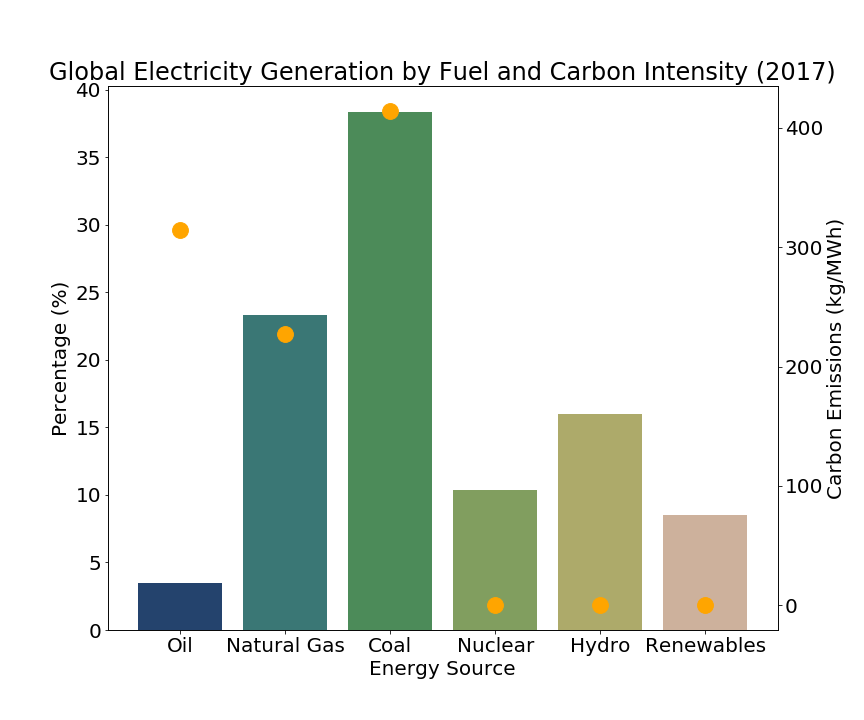
\includegraphics[width=0.45\textwidth]{figures/elec_gen_carbon.png}
		\caption{Global electricity generation sources and relative carbon emission intensity. ~\cite{BP2018,Hall1983}}
		\label{fig:fuel_emissions_market_share}
	\end{center}
\end{figure}


To achieve a low carbon energy infrastructure, and limit the effects of global warming, a transition in the electricity mix is required. Moving from a centralised and homogenous fossil fuel-based system to a distributed system based on renewable energy and batteries. Batteries are required due to the fact that most renewable sources are effected by conditions outside the control of the owners (e.g. time of day, wind speed and cloud cover). This leads to a need for electricity to be stored at times of low electricity demand and high renewable resources, and for the batteries to be discharged at times of high demand and low supply. 

Such a transition needs to be performed in a safe and non-disruptive manner -- it may be possible to close down all fossil fuel plants in the next year, though if this leads to electricity shortages and power cuts then this is likely to cause significant problems both for companies and homes. Therefore a stepped approach which allows seamless transfer is desirable. This may seem a simple process to achieve -- slowly phase out existing fossil fuel generators and replace these by renewable sources -- however, there are many risks and uncertainties in this process. Existing power plants have an expected lifetime and their owners wish to maximise this and the profits which can be made from them, renewable sources are still developing -- meaning that their efficiency and reliability will change in years to come.

Due to the long construction times, long operating periods and high costs of power plants, investment decisions made today can have long term impacts on future electricity supply \cite{Chappin2017}. Governments, and society, therefore have a role in ensuring that the negative externalities of pollution and carbon emission are priced into electricity generation so that optimal decisions are made. Due to the absence of central control in electricity generation investment, other methods must be used to influence the independent players of the electricity market. Methods such as carbon taxes, policy and regulation can aid in the goals of reducing carbon emissions to limit global warming, as agreed in the Paris agreement \cite{May2002}.

A common method to understand and reduce risk and uncertainty, especially in electricity planning, is simulation and modelling. Simulation and modelling allows practitioners to realise a physical system in a virtual model. In this context, a model is defined as an approximation of a system through the use of mathematical formulas and algorithms. Through simulation it is possible to test a system where real life experimentation would not be practical due to reasons such as prohibitively high costs, time constraints or risk of detrimental impacts. This has the dual benefit of minimising the risk of real decisions in the physical system, as well as allowing practitioners to test less risk-averse strategies. Without simulation one would frequently make safer decisions to reduce risk.

Agent-based modelling (ABM) is a class of computational simulation models composed of autonomous, interacting agents. ABMs are a way of modelling the dynamics of a complex system \cite{MacAl2010}. Due to the numerous and diverse actors involved in the generation, distribution and sale of electricity in liberalised electricity markets, agent based models are well suited and increasingly being used in the literature \cite{Zhou2007}.


In this paper, we present ElecSIM, an open-source agent-based model that simulates generation companies (GenCos) in an electricity market. ElecSIM models GenCos as multiple agents and electricity demand as a single aggregated agent, with a power exchange that facilitates trades between the two. 

GenCos actively make bids for each of the power plants they own to match demand. Their bids are based on their costs to supply a single unit (1MWh) of electricity, known as their short run marginal cost (SRMC), which excludes capital and fixed costs. The power exchange links bids to supply based on merit-order, with priority to the cheapest bids first. GenCos then invest in power plants based on expected profitability of each option.


Through simulation we can evaluate many strategies in order to identify those most likely to achieve our goals of rapid but non-disruptive migration from fossil to renewable.






ElecSIM can be used by:
\begin{itemize}
	\item {\bf Policy experts} to test policy outcomes under different scenarios and provide quantitative advice to policy makers. They can provide a simple script defining the policies they wish to use along with the parameters for these polices.
	\item {\bf Energy market developers} who can use the extensible framework to add such things as new energy sources, policy types, consumer profiles and storage types. Thus allowing ElecSIM to adapt to a changing ecosystem.
\end{itemize}




 {\color{red} A diagram showing the different players, who can influence them and how?}

This paper details our model, ElecSIM. We contribute a new open-source framework, and test different scenarios with varying carbon taxes to provide advice to stakeholders. Section \ref{Literature Review} is a literature review of the models currently used in practice. Section \ref{Model} details the model and assumptions made, and section \ref{Valdiation and Performance} details how we validated our model, and displays performance metrics. Section \ref{Scenario Testing} details our results, and explores ways in which ElecSIM can be used. We conclude the work and propose future work in section \ref{Conclusion}.




%
%To achieve carbon neutrality, this electricity mix must shift from a largely fossil fuel based system, to one based on renewable energy. We must use solar, wind and tidal power to generate electricity to power homes, industry and transport \cite{Hoffert2002}. Electricity is a significant proportion of our energy consumption -- consuming 22\% of energy usage per year -- which must grow to meet the demands of a low-carbon transport and heating system \cite{Lakshmi2017}.  Although other forms of energy consumption are important we focus here only on the production and consumption of electricity. 


%\begin{itemize}
%	\item We have developed a framework for evaluating alternative scenarios, prior to implementation of policy.
%	\item Used by experts working in collaboration with policy makers.
%	\item Importance of a transition in electricity infrastructure (Paris agreement, UK Climate change act)
%	\item Importance of understanding effect of decisions made today on the future (limit of 1.5C by 2050)
%	\item Introduce ElecSIM as a toolkit to inform long-term domestic policy questions in the electricity market. 
%	\item Ability to model the effects of carbon taxation, and the effect of different scenarios 
%	\item Talk about the need to model a non-stationary, dynamic system, with multiple interacting agents with imperfect information
%	\item Requirement for an Open-Source, free Toolkit written in python. Low barrier of entry, and integration with existing python data analytics and machine learning techniques. Transparent, reproducible, and data made available. This allows for results to be open to greater criticism and better inform policy decisions.
%	\item Simple model which matches real life behaviour for low complexity and therefore increases transparency.
%\end{itemize}



\section{Literature Review}\label{Literature Review}
Live experimentation of physical processes is often not practical. The costs of real life experimentation can be prohibitively high, and it normally requires significant time in order to fully ascertain the long-term trends. There is also a risk that changes can have detrimental impacts ~\cite{Forshaw2016}. These factors are particularly true for an electricity market, where decisions made can have long term impacts on energy mix, carbon emissions and agent behaviour.  A solution to this is simulation, which can be used for rapid testing and prototyping of ideas. Simulation is the substitution of a physical process with a computer model. The computer model is parametrised by real world data and phenomena. The user is then able to experiment using this model, and assess the likelihoods of outcomes under certain scenarios and input variables \cite{Law:603360}.

Energy policy modelling is an example where simulation can be used. Real-life experimentation of energy policy is not always feasible, and as discussed, decisions can have long-term impacts. A number of different simulations and computer models have been used to aid policy makers and energy market developers in coming to informed conclusions.

Energy models can typically be classified as top-down macro-economic models or bottom-up techno-economic models~\cite{Bohringer1998}. Top-down models generally focus on behavioural realism with a focus on macro-economic metrics. They are useful for studying economy-wide responses to policies. ~\cite{Hall2016}, for example MARKAL-MACRO \cite{Fishbone1981} and LEAP \cite{Heaps2016}. Bottom-up models represent the energy sector in detail, and are written as mathematical programming problems~\cite{Gargiulo2013}. They detail technology explicitly, and can include cost and emissions implications~\cite{Hall2016}.

It is possible to further categorise bottom-up models into optimisation and simulation models. Optimisation energy models minimise costs or maximise welfare from the perspective of a central planner, for instance a government~\cite{Keles2017}. A use-case would be a government that wants cheap, reliable and low-carbon electricity supply by a future date. An optimisation model would find the optimal mix of generators to meet this whilst taking into account the constraints. Examples of optimisation models are MARKAL/TIMES~\cite{Fishbone1981} and MESSAGE~\cite{Schrattenholzer1981}. MARKAL is possibly the most widely used general purpose energy systems model~\cite{Pfenninger2014}.

However, electricity market liberalisation in many Western democracies has changed the framework conditions. Centralised, monopolistic, decision making entities has given way to multiple heterogeneous agents acting in their own best interest~\cite{Most2010}. Therefore, certain policy options which encourage changes must be used by a central planner to attain a desired outcome, for example carbon taxes or subsidies. It is therefore proposed that these complex agents are modelled using agent-based modelling.

As a result of this, agent-based simulation has received increasing attention in recent years, and a number of simulation tools have emerged, for example SEPIA~\cite{Kraan2018} EMCAS~\cite{Conzelmann}, NEMSIM~\cite{Batten2006}, AMES~\cite{Sun2007}, PowerACE~\cite{Rothengatter2007}, MACSEM~\cite{Praca2003}, GAPEX~\cite{Cincotti2013} and  EMLab~\cite{Chappin2017}. However, none of which suit the needs of an open source, long-term market model which has a stochastic representation of input variables.

SEPIA \cite{Harp2000} is a discrete event agent based model which utilises Q-learning for agent behaviour. SEPIA models plants as being always on, and does not have an independent system operator (ISO), which in an electricity market, is an independent non-profit organization for coordinating and controlling of regular operations of the electric power system and market  \cite{Zhou2007}. SEPIA does not model a spot market, instead focusing on bilateral contracts. As opposed to this, ElecSIM has been designed with a merit-order, spot market in mind, with peaker power plants running at times of high demand, and renewable energy supply running intermittently.

EMCAS ~\cite{Conzelmann} is a closed source agent-based framework which investigates the interactions between physical infrastructures and economic behaviour of market participants. ElecSIM, however, focuses on purely the dynamics on the market, with an aim of providing a simplified, transparent, open source model of market operation, whilst maintaining robustness.

PowerACE ~\cite{Rothengatter2007} is also a closed source agent-based simulation of electricity markets that integrates short-term perspectives of daily electricity trading and long-term investment decisions. Similarly to ElecSIM, PowerACE initialises agents with all power plants in their respective country. However, unlike ElecSIM, PowerACE does not take into account stochasticity of price risks in electricity markets which is of crucial importance to real markets~\cite{Most2010}.

EMLab ~\cite{Chappin2017} is also an agent-based modelling toolkit for the electricity market. EMLab models an endogenous European emissions trading scheme with a yearly time-step. However, like PowerACE, EMLab differs from ElecSIM by not taking into account stochasticity in the electricity markets, such as outages, differing fuel prices within a year period and stochasticity in power plant operating costs. However, after correspondence with the authors, we were unable to run EMLab.

AMES ~\cite{Sun2007} is an agent-based model specific to the US Wholesale Power Market Platform. GAPEX \cite{Cincotti2013} is an agent-based framework for modelling and simulating power exchanges in MATLAB . GAPEX utilises an enhanced version of the reinforcement technique Roth-Erev to consider the presence of affine total cost functions. However, neither of these model the long-term dynamics that ElecSIM is designed for.

We therefore propose ElecSIM to fill a gap of an open source, long-term stochastic investment, agent-based model. {\color{red}Table with ticks and crosses to show desired features and which ones have them?}

\begin{itemize}
	\item Agent Based Models - eg. EMCAS, PowerACE, EMLab: Leaves a requirement for an open source toolkit written in python. Many one-off models available, however difficult to apply to different scenarios.
	(SEPIA [6], EMCAS [7], NEMSIM [8], AMES [9], PowerACE [10], MASCEM [11, 12], and GAPEX [13] \cite{Lopes})
	\item Bottom-up optimization models to find minimum cost of electricity system. \cite{Pfenninger2014}. eg. MARKAL/TIMES, MESSAGE. (These do not provide information on how to achieve a certain goal, particularly in a liberalized energy market. Or scenarios as to why a goal may not be achieved as the goal is assumed to be achieved.)
	\item Computational general equilibrium (CGE) models - Top-down macroeconomic models partial equilibrium model (energy supply, demand, cross-border trade, emissions)- Can be highly complex and difficult to understand. eg. NEMS, PRIMES.
\end{itemize}




\section{ElecSIM Architecture} \label{Model}

ElecSIM has been designed for ease of use to enable non-experts to rapidly test policies and observe the outcomes of various scenarios such as demand growth. The user is able to input exogenous variables such as fuel costs, carbon taxes, power plants, power plant costs and electricity demand. This allows for the initialisation of different countries and scenarios to be tested.


\subsection{Overview}

\begin{figure}[b]
	\centering
	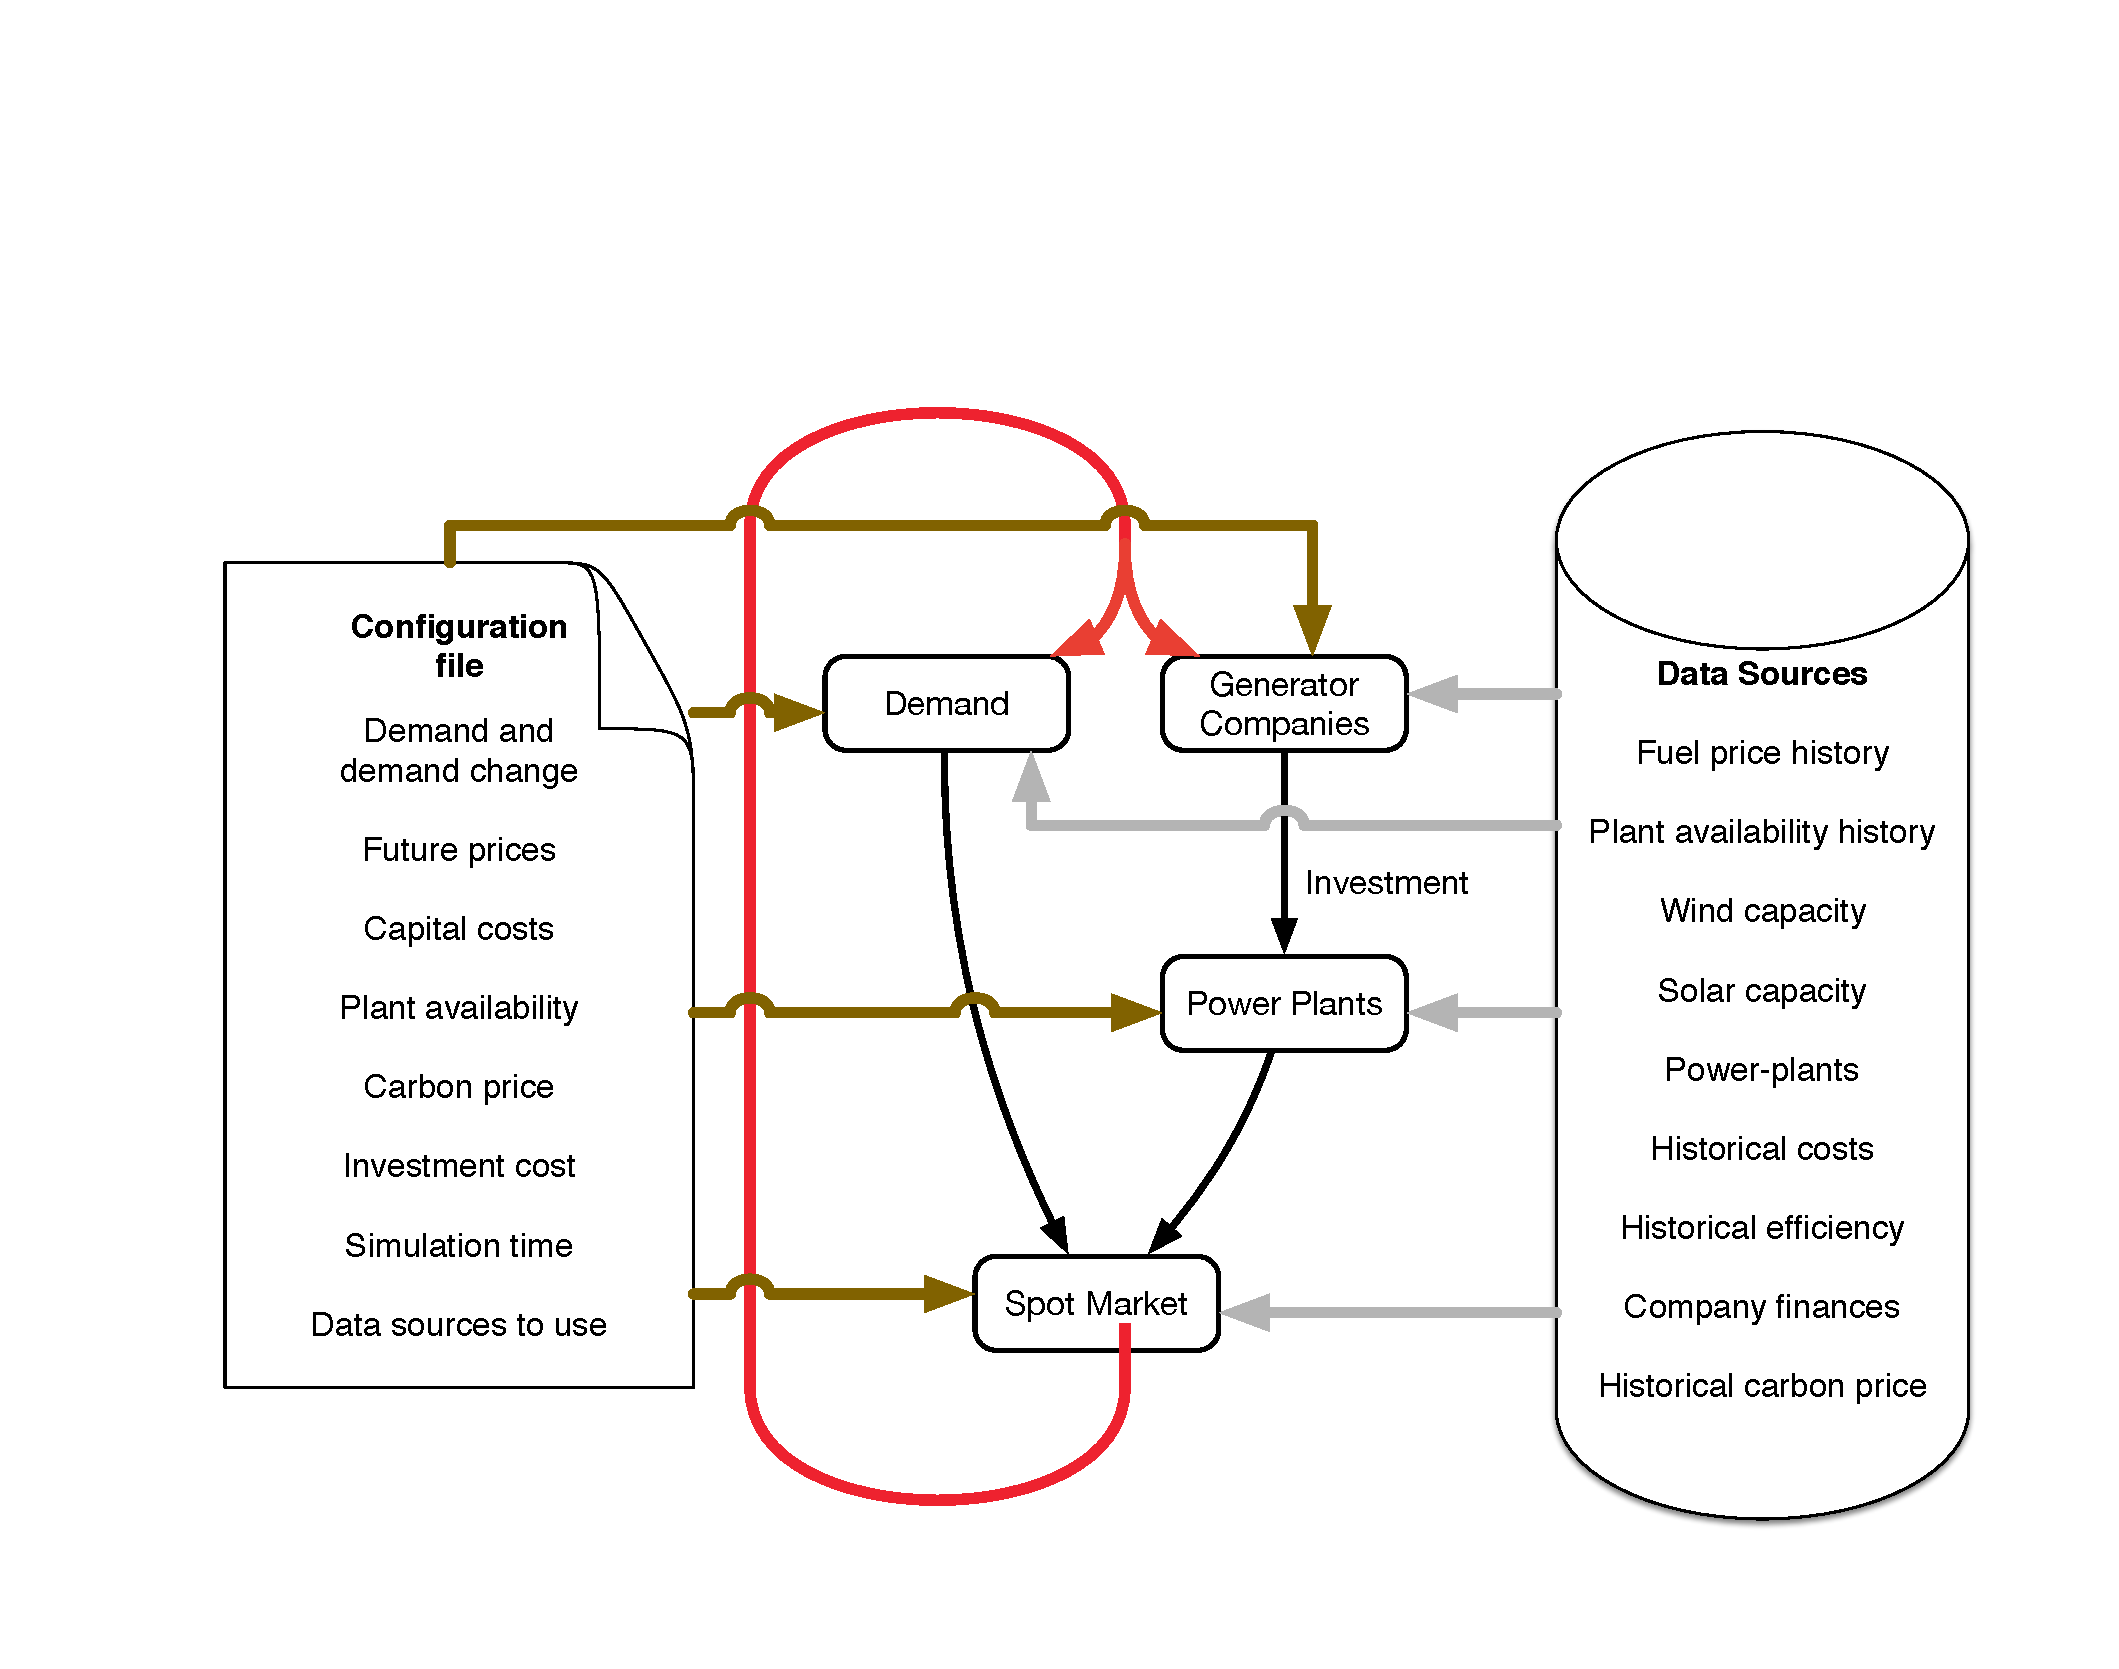
\includegraphics[width=0.97\linewidth]{figures/System_overview}
	\caption{High level system overview demonstrating fundamental parts of ElecSIM.}
	\label{fig:systemoverview}
\end{figure}




ElecSIM is made up of four fundamental parts: The agents, which are split up into demand and generation companies (GenCos) . Power plants which are owned by the GenCos. A Power Exchange which controls a spot market to match GenCo owned power plants with electricity demand, and the world in which these agents and market exist.

A schematic of ElecSIM is displayed in Figure \ref{fig:systemoverview} which displays these four fundamental sections and demonstrates how they interact.

\subsubsection{Data parametrisation} To parametrise the world ElecSIM contains a configuration file and a collection of data sources. These data sources contain information such as historical fuel prices, historical plant availability, wind and solar capacity, power plant costs, historical costs, historical efficiency, company finances and historical carbon price. This is data that does not change from scenario to scenario, however can vary between countries.

The configuration file allows for rapid changes to test different hypothesis and scenarios, and points to previously mentioned data sources. The configuration file enables the changing of demand growth and shape,  future fuel and carbon prices, capital costs, plant availability, investment costs and simulation time. These data is used to calibrate the world.

\subsubsection{Demand Agent}
The demand agent is a simplified representation of aggregated demand in a particular county. The demand is represented as a load duration curve. An example load duration curve for a year is demonstrated in Figure \ref{fig:loaddurationcurve}. A load duration curve is an arrangement of all load levels in descending order of magnitude, where the lowest segment demand demonstrates baseload (ie. 100\% of time), and the highest segment represents peak demand. Each year, the demand agent multiplies the percentage of change in demand with each segment of the load duration curve. Therefore, whilst total demand changes between years, the ratio between each segment of the load duration curve is assumed not to change.

\begin{figure}
	\centering
	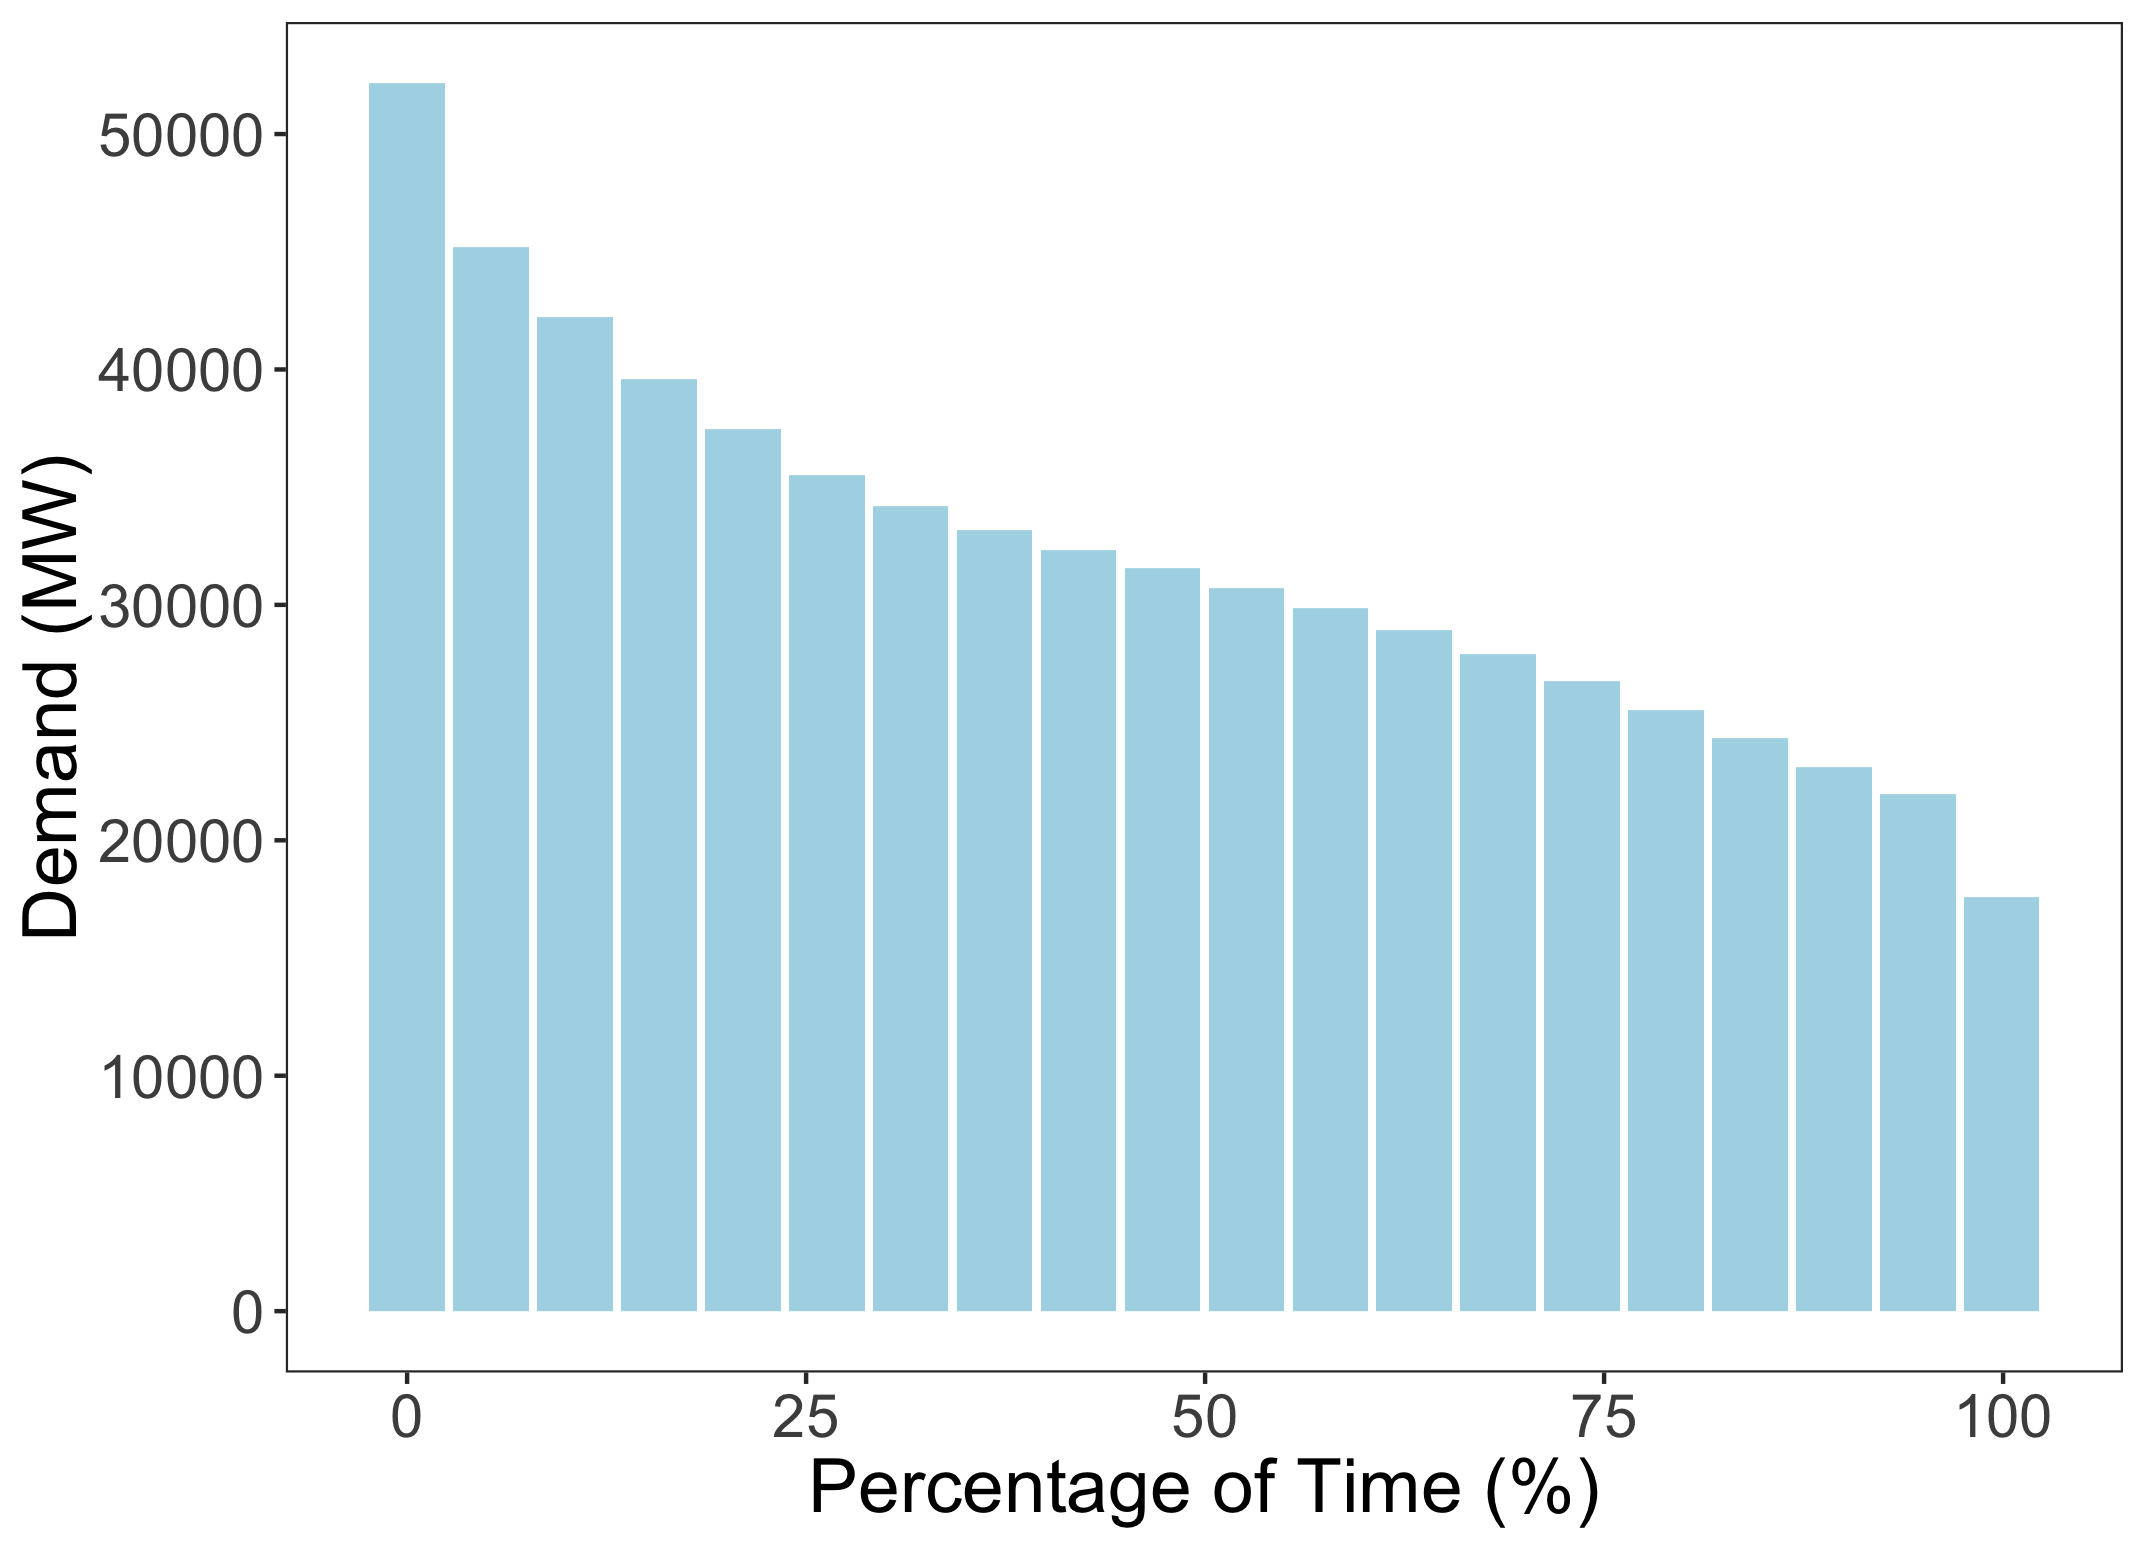
\includegraphics[width=0.95\linewidth]{figures/load_duration_curve}
	\caption{Example load duration curve in a single year.}
	\label{fig:loaddurationcurve}
\end{figure}

As per \cite{Chappin2017}, we modelled the load duration curve of the electricity demand for one year with twenty segments. Twenty segments enabled us to capture the varying demand of electricity throughout the year to a high enough degree of accuracy, whilst also reducing computational complexity. 


\subsubsection{Generation Company Agents} The GenCos have two main functions. Investing in power plants and making bids to sell their electricity each year for every one of their power plants. We will first focus on the buying and selling of electricity using a Power Exchange, and then cover the investment algorithm for GenCos.

\subsubsection{Electricity Market} \label{sssec:electricity_market} A simulated electricity market is run every year, where electricity is bought and sold on an electricity spot market. Figure \ref{fig:powermarket} displays the market process for each segment of demand. Power plants bid the short run marginal cost (SRMC) of each power plant. SRMC is the price that it costs a generator to sell a unit of electrical power (1MWh) excluding fixed and capital costs. 

The power exchange sorts bids in order of price, as is shown in Figure \ref{fig:powermarket}, and accepts the lowest bids until supply meets demand. Once supply meets demand, the spot price or system marginal price (SMP) is paid to all generators regardless of their initial bid. It is for this reason that generators are motivated to bid their SRMC, to ensure that their generator is being utilised, and reducing the risk of over bidding and not being selected.

Higher segments of demand command higher prices, due to more expensive generators being selected to meet demand. This leads to a price duration curve.
 

\begin{figure}
	\centering
	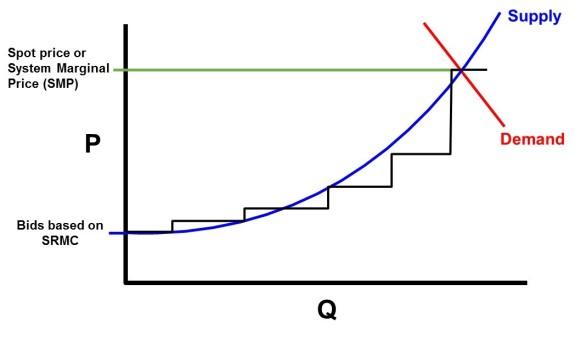
\includegraphics[width=1\linewidth]{figures/power_market}
	\caption{Power exchange clearing \cite{nuclear_economics_consulting_group_2019}.}
	\label{fig:powermarket}
\end{figure}

\subsubsection{Investment}




Investment in power plants is made based upon a net present value (NPV) calculation. NPV is a summation of the present value of a series of present and future cash flow. NPV provides a method for evaluating and comparing investments with cash flows spread over many years, making it suited to evaluating power plants which have a long lifetime. NPV is based upon the fact that current cash flow is worth more than future cash flow. This is due to the fact that money today can be invested and have a rate of return. This means that, for example \$50,000 today is worth more than \$50,000 in 10 years time.

Equation \ref{eq:npv_eq} displays the calculation of NPV. Where $t$ is the year of the cash flow. $i$ is the discount rate, $N$ is total number of periods, or lifetime of power plant, and $R_t$ is the net cash flow (cash inflow minus cash outflow) at time $t$.

\begin{equation} \label{eq:npv_eq}
NPV(i, N) = \sum_{t=0}^{N}\frac{R_t}{(1+t)^t}
\end{equation}

A discount rate set by a firm's weighted average cost of capital (WACC) is often used. Where WACC is the rate that a company is expected to pay on average for its stock and debt. However, it is often believed that a higher rate should be selected to adjust for differing risk profiles, opportunity cost and rate of return desired.

Data is available for average WACC for power plants, and can be set in the configuration file. However, to account for differing risk profiles, opportunity costs, rate of return desired, and WACC based on companies' relative credit risk, we have sampled difference in discount rates from the mean WACC with a Gaussian distribution with a standard deviation of $\pm3\%$. Which was chosen to give sufficient variance between GenCos whilst remaining close to the mean set by the user.

To calculate the expected return per year of a power plant, an understanding of future market conditions is required. Future market conditions are dependent on demand and costs that would be incurred by the GenCo based upon each prospective investment. We simplify this calculation by forecasting $N$ years into the future, which can be selected by the user. We assume that this year is representative of each year of a power plant's lifetime.

As in the real world, GenCos have imperfect information, and therefore must forecast expected demand, fuel prices, carbon price and electricity sale price. This achieved by fitting functions to historical data. Each GenCo is different in that they will use differing historical time periods of data to forecast in the future. The distribution of this is configurable in the configuration file, referred to in Figure \ref{fig:systemoverview}.

Fuel price and carbon price is forecast using a linear regression. Demand, however, is first forecast using an exponential function, to take into account compounded growth. If a reasonable fit for historical demand data can not be found with optimisation, linear regression is used.

These forecasted data is then used to simulate a market $N$ years into the future using the same electricity market algorithm that is detailed in Section \ref{sssec:electricity_market}. We simulate a market based on the expected bids -- based on SRMC -- that every operating power plant will make. This includes the removal of plants that will be past their operating period, and the introduction of plants that are in construction or pre-development stages. 

However, there may be scenarios where demand is forecast to grow significantly, and limited investments have, at this point, been made to meet demand at $N$ years into the future. The expected price, would therefore be calculated to be that of lost load. Where lost load is defined as the price customers would be willing to pay to avoid disruption in their electricity supply. To avoid GenCos from predicting that large profits will be made, and under the assumption that further power plant investments will be made by other GenCos, the lost load price is replaced with a predicted electricity price using a linear regression based on prices at lower points of the demand curve. If zero segments of demand are met, then the lost load price is used to encourage significant investment, whilst if only a single segment of demand is met then the price of this demand segment is chosen.

Once expected fuel prices, carbon price, discount rate, and expected sale price of electricity are all forecast, the NPV can be calculated. GenCos must typically provide a certain percentage of upfront capital, with the rest coming from investors in the form of stock and shares or debt (WACC). The percentage of upfront capital, or down payment, is set at $25\%$, but can be customised by the user in the configuration file. The GenCos then invest in the power plant with the highest NPV that they can afford, and this is repeated until they can no longer afford any more plants. We make this assumption as the NPV calculation provides information based upon risk profile and required rate of return.

\subsection{Power Plant Parameters}



The estimation of power plant parameters is critical to electricity market models. Costs form an important element of markets and investment, and publicly available data for individual countries can be scarce. Thus, extrapolation and interpolation is required to estimate costs for power plants of differing sizes, types and years of construction.

We enable users to initialise costs relevant to their particular country. They can provide highly detailed costs, with the parameters shown in Table \ref{table:parameter_notation}, or an average cost per MWh produced over the lifetime of a plant, also known as levelised cost of electricty (LCOE).

The parameters in Table \ref{table:parameter_notation} are explained here: Efficiency ($\eta$) is defined as the percentage of energy from fuel that is converted into electrical energy. Operating period ($OP$) is the total period in which a power plant is in operation. Pre-development period ($P_D$) and pre-development costs ($P_C$) include the time and costs for pre-licensing, technical and design, as well as costs incurred due to regulatory, licensing and public enquiry. The construction period ($C_D$) and construction costs ($C_C$) are incurred during the development of the plant, excluding network connections. The infrastructure costs ($I_C$) are the costs incurred by the developer in connecting the plant to the electricity or gas grid. Fixed operation \& maintenance costs ($F_C$) are costs incurred in operating the plant that do not vary based on plant output. Variable operation \& maintenance ($V_C$) costs are costs incurred in operating the plant that do depend on generator output \cite{Ltd2016}.



\begin{table}[h]
	\centering
	\csvautobooktabular{tables/notation_formated.csv}
	\caption{Parameter notation.}
	\label{table:parameter_notation}
\end{table}

Precise data is often available only for specific sized plants. Estimating the individual costs of power plants between two known capacities is achieved through linear interpolation of each parameter. When the plant to be estimated falls outside of the range of known data points the closest data point is used. For example, the parameters of a $1,500$MW combined cycle gas plant (CCGT) are estimated to be the same as a $1,200$MW CCGT plant if the $1,200$MW plant was the largest available data point. 

If specific parameters are not known (those referred to in Table \ref{table:parameter_notation}), then the LCOE can be used for estimation, provided that these parameters are available for a single instance of each type of power plant. This is achieved through linear optimisation, with constraints available for each of the parameters. These constraints can be set by the user, enabling, for example, varying operation and maintenance costs per country as a fraction of the levelised cost of electricity.


In addition to cost parameters, the availability and capacity factors are required to fully parametrise power plants. Availability is the percentage of time that a power plant could possibly produce electricity over a given time period. Availability can be reduced by forced and planned outages. Historical data is also required, due to the fact that older plants have lower availability factors than newer plants.

Capacity factor is the actual electrical energy produced over a given time period divided by the maximum possible electrical energy it could have produced. In contrast to availability, capacity factor can be impacted by regulatory constraints, market forces and resource availability. For solar and wind, capacity factors can change significantly with time. Higher capacity factors are common for solar installations in the summer, and lower in winter for example \cite{Stoft2002}. 

To model the intermittency of wind and solar power we allow them to contribute only a certain percentage of their total capacity (nameplate capacity) for each load segment. This percentage is based upon empirical wind and solar capacity factors, relating demand to average capacity \cite{Pfenninger2016, Staffell2016, Chappin2017}. This is done as there is a correlation between demand and wind speed, as well as with solar irradiance. The requirement of storage to provide constant electricity from intermittent resources is an important issue. However, due to the fact that ElecSIM takes yearly time steps, we are unable to model short term variability in electricity demand. We also, do not model long-term storage due to its currently limited ability. 

When initialised, the variable operation and maintenance costs are selected from a uniform distribution, with the ability for the user to set maximum percentage increase or decrease. A uniform distribution was chosen to capture the large deviations that can occur in variation of variable operation and maintenance, especially other a long time period. By doing this, the variance in costs between individual power plants for processes such as preventative and corrective maintenance, labour costs and skill, health and safety and chance are different per plant instant.  

Whilst fuel price is controlled by the user, there is inherent volatility in fuel price in a single year. To take into account this variability, an ARIMA model was fit to historical gas and coal price data. The standard deviation of the residuals was used to model the precise price of fuel that a generation company will buy the fuel in a given year. This takes into account differences in hedging strategies and the process of luck between competing generation companies.

With historical power plants which have been refurbished, we sample their initialisation randomly between 15 years prior to initialisation year and the initialisation year.

\subsubsection{World}

Figure \ref{fig:lowlevelsystem} demonstrates the world and how it is co-ordinates data and processes. It contains information on every single GenCo, Power Exchange, and runs processes. It also contains information on the year number and collects simulation data.

The world brings together power plant data on one side and demand data on the other. The investment decisions are based upon future demand and power plant costs. The merit order bids are based upon the investment decisions made and power plant costs.

Exogenous variables include fuel and \ce{CO2} prices as well as demand growth. Once the data is initialised the world calls on the Power Exchange to operate the yearly electricity spot market.

The world dismantles old plants once they have reached the end of their lifetime. Power plants are taken out of service if they have not sold any electricity in the past 7 years. We decided upon this due to the fact that power generators have high, sunk capital costs, which often have high demolition costs. We assume, therefore, that generator companies are willing to wait circa $\frac{1}{4}$ of their lives to see if a pay-out occurs due to the breakdown of competing power plants, increasing demand, or governmental support in the form of a carbon tax increase or reduction.

The world also settles the accounts of the GenCos, by paying bids, and removing operating and capital costs as well as loan and dividend payments.

\begin{figure*}
	\centering
	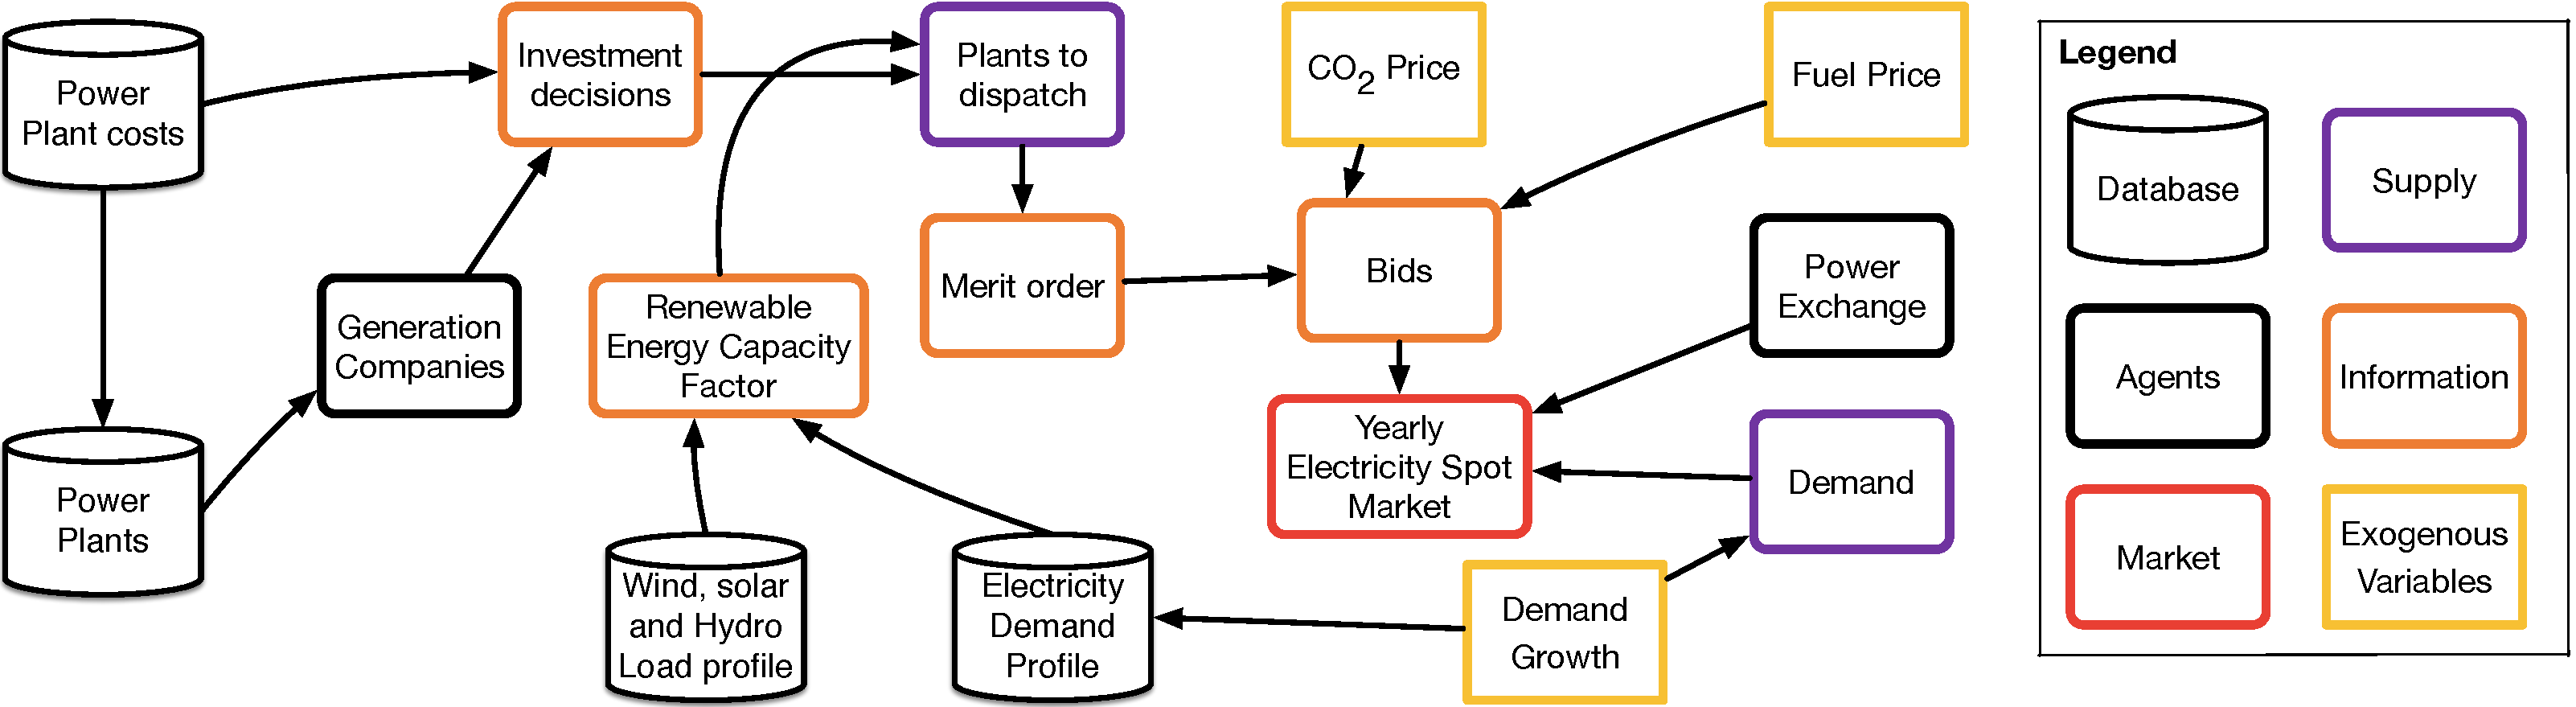
\includegraphics[width=0.97\linewidth]{figures/low_level_system}
	\caption{ElecSIM simulation overview}
	\label{fig:lowlevelsystem}
\end{figure*}


%GenCos  invest in power plants based on the highest positive net present value (NPV). Bids are made for each power plant based on the power plants short run marginal cost. A Power Exchange operator matches these bids with demand in merit order. 



%\begin{figure}[h]
%	\begin{center}
%		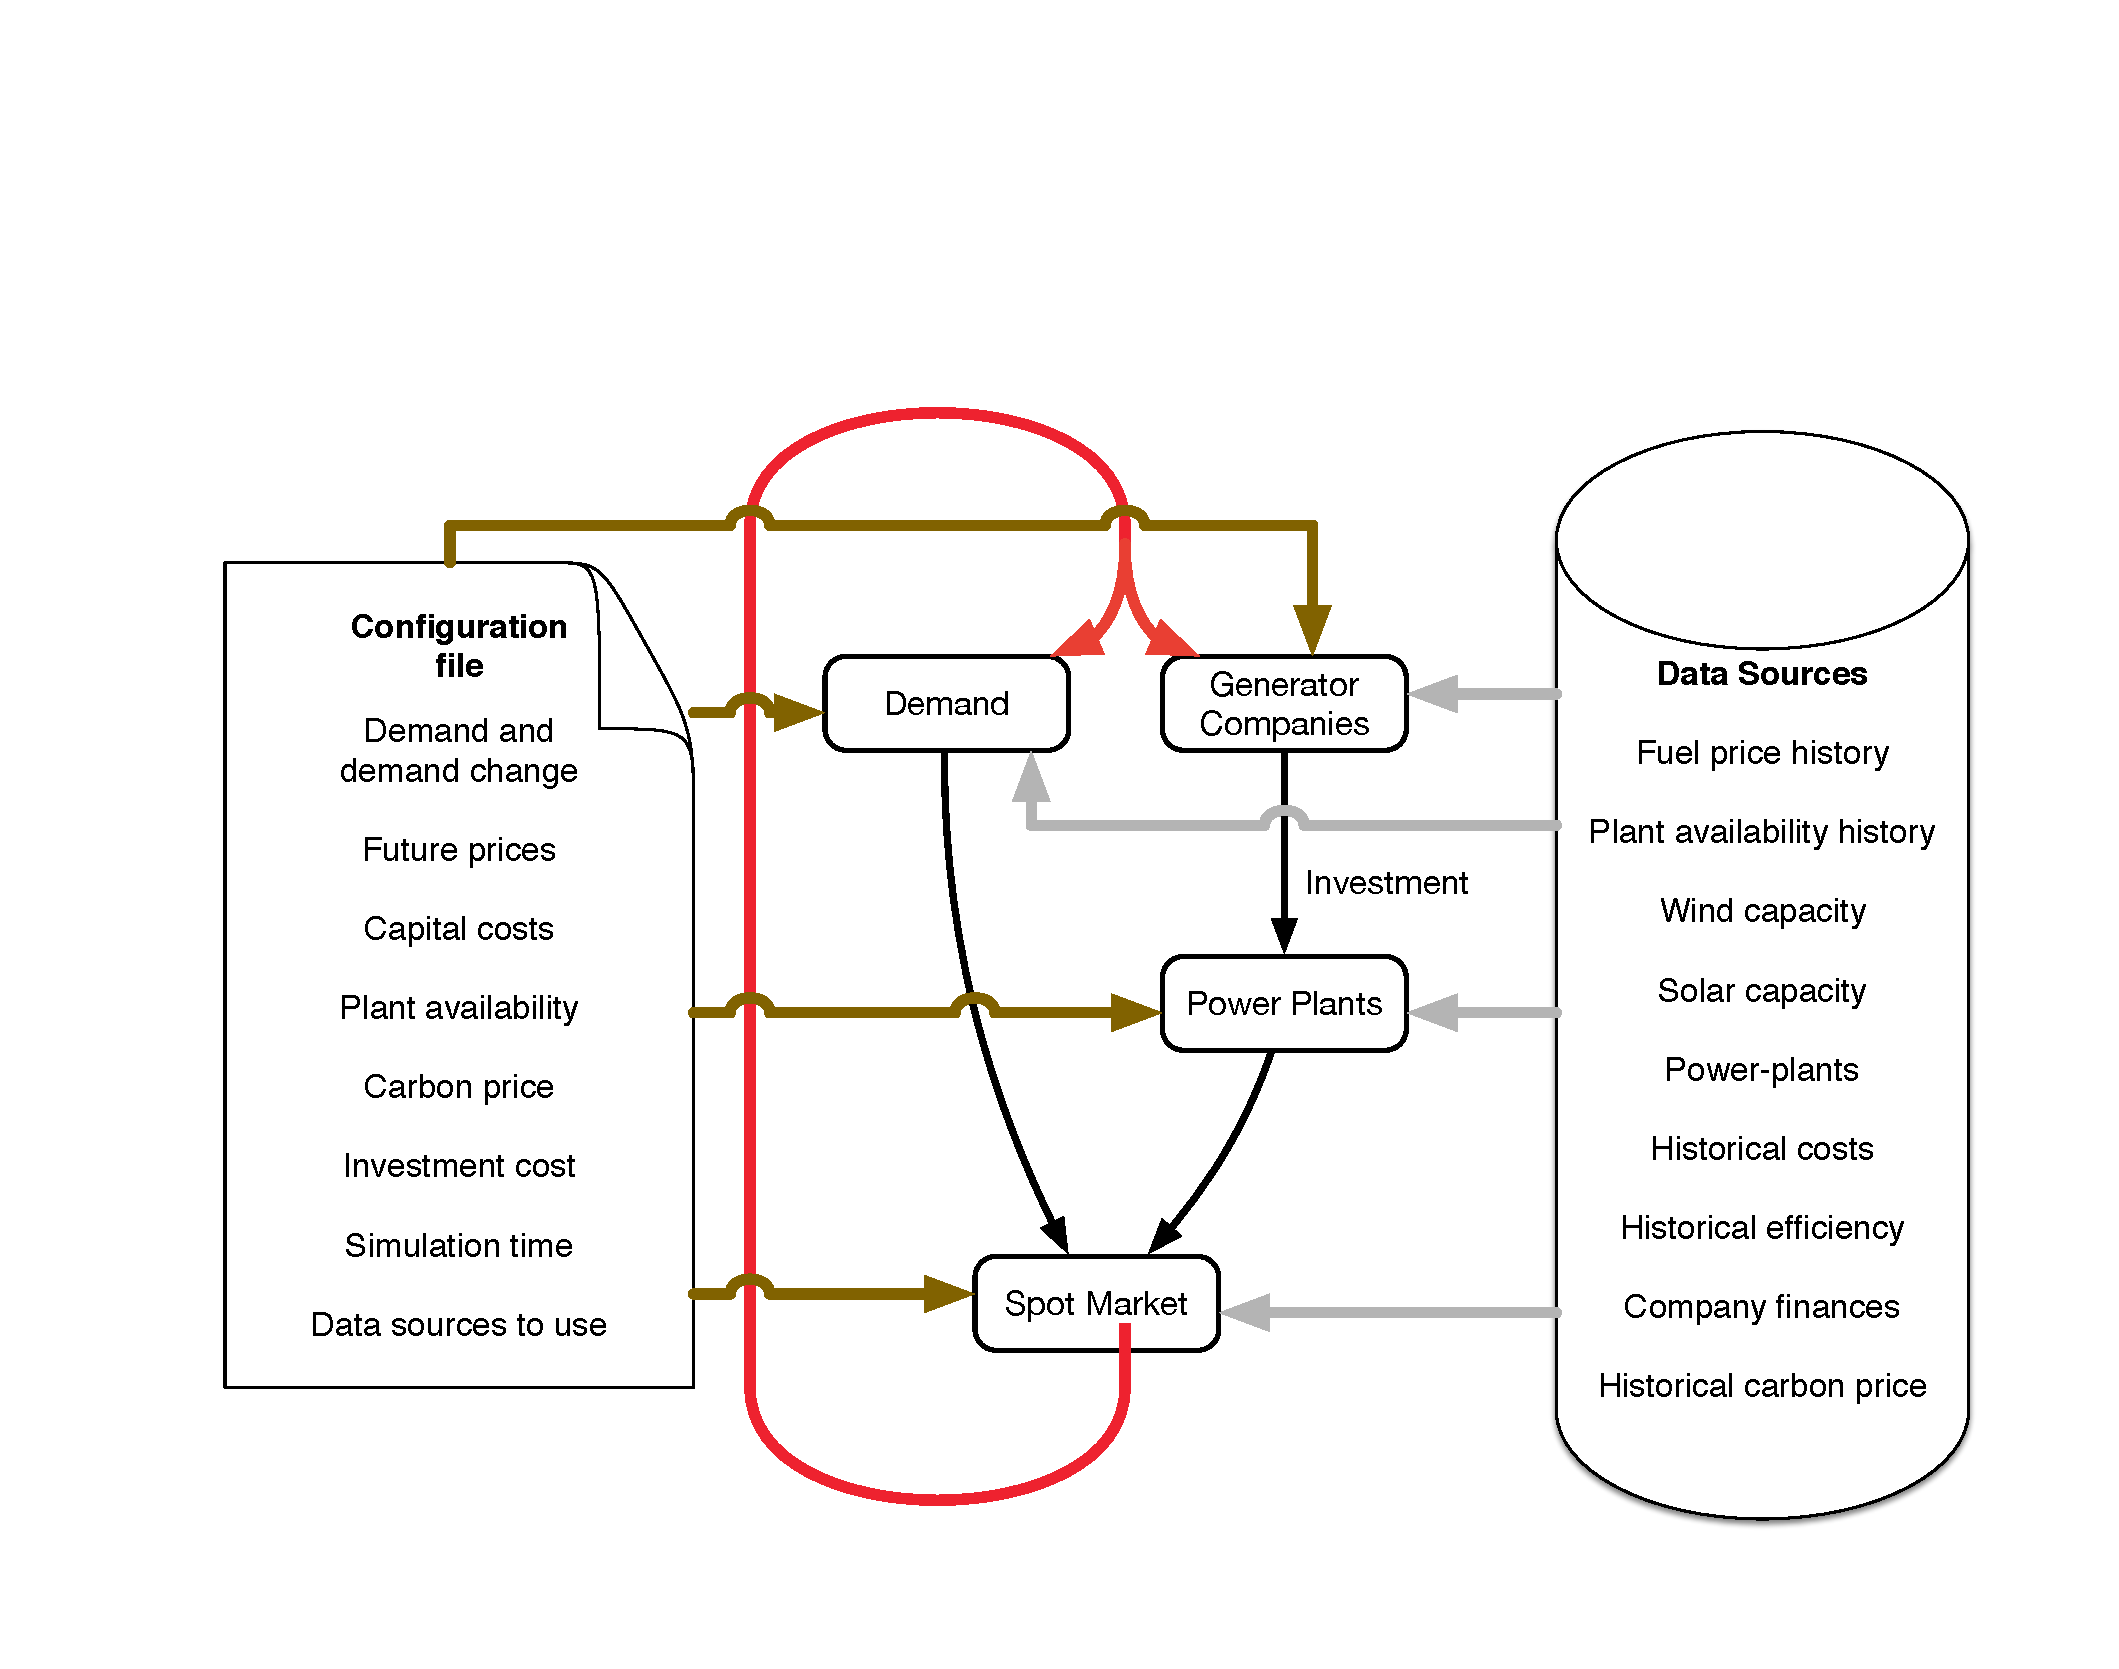
\includegraphics[width=0.5\textwidth]{figures/System_overview.pdf}
%		\caption{ElecSIM simulation overview.}
%		\label{fig:system_overview}
%	\end{center}
%\end{figure}




\subsection{UK Case Study}

Here we study a realisation of ElecSIM, which we calibrated to the United Kingdom.

around a mean of 10\% for nuclear power plants \cite{Paper2012} and 5.9\% for all other generators \cite{KPMG2017}.





\subsubsection{Data Initialisation}ElecSIM's power generation costs are initialised using the UK government Department for Business, Energy and Industrial Strategy (BEIS) power plant generation report \cite{Department2016}. This contains information on power plants found in Table \ref{table:parameter_notation}.

For historical power plants, we used historical costs of Levelised Cost of Energy (LCOE) \cite{Dale2013}. Each parameter was scaled linearly from the modern LCOE calculated from the BEIS report, to attain the relevant historical LCOE. In this realisation we ensured that each of the parameters were scaled linearly to the modern power plant costs found in \cite{Department2016}. Historical plant efficiency was taken into account for gas and coal power plants using data from the USA \cite{EIA2013}.

To model variance in gas and coal prices we used data from \cite{coalprices,gasprices}.

Outages are modelled by using availability data of gas, coal, photovoltaic, offshore and onshore power generators \cite{Ltd2016, Hunt2015, carroll-j}. Historical availabilities are modelled for older gas, coal and hydro power plants \cite{AlbertaSystemElectricOperator2016}.






\subsubsection{Spot Market}

The lost load is set to be \textsterling6000 to encourage investment as per the recommendations of the UK government \cite{DECC2013}.

\subsubsection{Investment}

As agents are modelled to have imperfect information, we model that they make prediction on future electricity and \ce{CO2} prices, as well as demand change. Each generation company has a different look-back period sampled uniformly from the previous 3 to 7 years.


The cost of equity and debt is modelled as a weighted average cost of capital (WACC), with values of 5.9\% for non-nuclear power plants, and 10\% for nuclear power plants \cite{KPMG2017, Paper2012}. The WACC is used as the discount rate for net present value calculations \cite{KincheloeStephenC1990TWAC}. 





%
%\begin{itemize}
%	\item Model can be modified through a single python scenario file which includes exogenous variables such as number of generation companies, power plants, power plant costs, tax and fuel prices, and demand.
%	\item Architectural framework:
%	\begin{itemize}
%		\item Agents are generation companies.
%		\item Generation companies initialized from government data. And randomized discount rate around a mean of 10\% for nuclear power plants and 5.9\% for other types of generators.
%		\item Costs of power plants taken from empirical data. 
%		\item Historical LCOE costs taken from data, with individual costs such as fixed operation and maintenance, construction and pre-development costs scaled linearly to match LCOE value. (This can be changed by user by specifying linear optimisation constraints).
%		\item Historical Gas turbine and Coal plant efficiency taken from epa data.
%		\item Variable operation and maintenance costs are stochastic to take into account differences in design types, preventative and corrective maintenance, labour costs and skill, asset and site management, health and safety and chance.
%		\item Electricity demand taken from historical data and split up into 19 load segments.
%		\item CO2 prices, fuel Prices, demand growth are exogenous
%		\item Fuel is bought by power producers each year at different prices, related to the standard deviation from historical data. This simulates different hedging strategies, luck and timing of fuel purchasing.
%		\item Outages are modelled by assuming a 93\% outage rate for fuel plants \cite{Ltd2016} and 97\% outage for renewables. \cite{carroll-j}
%		\item Generation companies bid their short run marginal costs.
%		\item Investments made on highest Net Present Value results. CO2 price, fuel price and demand are predicted 7 years ahead using linear regression. 
%		\item Estimated sale of electricity price calculated by simulating a market 7 years into the future with expected power plants that are running and have been taken out of service.
%		\item Investors will only invest if they have 25\% of the total upfront costs. (the rest taken on by debt and equity as assumed by WACC value.)
%		\item Intermittent power generators can only submit a certain percentage of their total capacity for each load segment. This percentage is matched with empirical data.
%		\item Bids accepted by a centralised Power Exchange based on merit order. Generation companies bid their short run marginal cost.
%	\end{itemize}
%	\item Assumptions: 
%	\begin{itemize}
%		\item Yearly time step
%		\item Renewables contribute to load curve of each demand segment matched with empirical data of typical wind and solar availability at each demand segment
%		\item Different discount rates per user (randomized)
%		\item Country initialized with full amount of power plants and generation companies in country and total demand data considered
%		\item No curtailment of renewables
%		\item Imperfect foresight - Prediction required for demand, co2 price, fuel cost, other investments.
%		\item Power plant construction and pre-development periods and costs modelled from UK Government BEIS data
%		\item Investments based on highest NPV using a single year 7 (can be changed in scenario file) time steps into the future to predict all years of power plant.
%		\item Agents predict next year's fuel, carbon and demand using linear regression and randomized look back period (between 3 and 6.)
%		\item Plants are dismantled after their lifetime, and only enter operation after pre-development/construction.
%		\item Legacy power plants are reinitialized to random starting year to account for refurbishment.
%		\end{itemize}
%\end{itemize}

\section{Validation and Performance}\label{Valdiation and Performance}

\subsection{Validation} Validation of models is important to ascertain that the results are accurate. However, it should be noted that these long-term simulations are not predictions of the future, rather possible outcomes based upon certain assumptions. Therefore, the results from ElecSIM should be analysed by understanding the underlying assumptions of the model, and comparing inputs to outcomes.

Jager posits that a certain outcome or development path, captured by empirical data, might have developed in a completely different direction due to chance \cite{Jager2006a}. However, through observation, the processes that emerge from a model should be realistic and in keeping with expected behaviour \cite{Jager2006}.

We begin by comparing the price duration curve in the year 2018. Figure \ref{fig:price_duration_curve} shows the N2EX Day Ahead Auction Prices of the UK \cite{nordpool_2019}, the stochastic simulated electricity prices, and the non-stochastic electricity price throughout the year 2018.

Table \ref{table:validation_metrics} shows performance metrics of the stochastic and non-stochastic runs versus the actual price duration curve. It can be seen that stochastic implementation (ElecSIM), improves the mean absolute error (MAE) by $52.5\%$.

Therefore, the adding of stochasticity to fuel prices and variable operation \& maintenance improves on previous attempts of a yearly step model.

By observing the processes that emerge from the long-term scenarios, we can see that carbon price and investment in renewable generation are positively correlated, and is what one would expect.

We found that the net present value (NPV) calculations are realistic, with onshore wind and Combined Cycle Gas Turbines (CCGT) the technologies that are most invested in. It is true, within the United Kingdom, that Onshore wind and CCGT power generators are the most cost effective, and heavy government subsidies are required for other generation types such as nuclear and coal. 

\begin{figure}[H]
	\begin{center}
		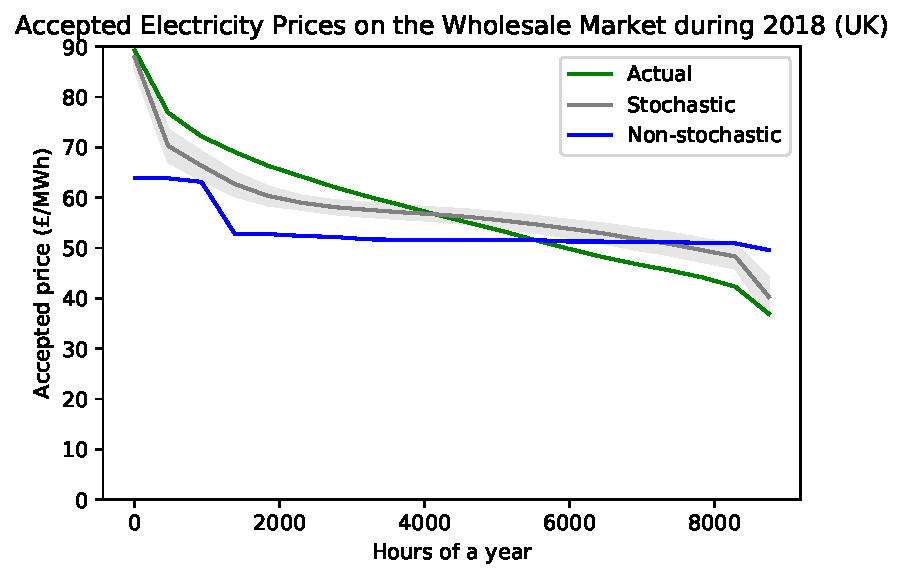
\includegraphics[width=0.5\textwidth]{figures/load_price_duration_curve_comparison.pdf}
		\caption{Price duration curve which compares real electricity prices to those paid in ElecSIM with stochasticity (40 runs) and no stochasticity.}
		\label{fig:price_duration_curve}
	\end{center}
\end{figure}

\begin{table}[h]
	\centering
	\csvautobooktabular{tables/validation/initialisation_run_validation.csv}
	\caption{Validation performance metrics.}
	\label{table:validation_metrics}
\end{table}

\subsection{Performance and Implementation}

ElecSIM was built using python, this enabled us to lower barriers to entry and allow for users to integrate state-of-the-art machine learning and statistical packages in future work. We used project mesa as an open source agent based modelling framework for its ease of use \cite{Masad2015}.

 We utilised Microsoft Azure Public Cloud. We used two virtual machines of 64 vCPU's each (D64 v3), which are built using Intel Broadwell E5-2673 v4 2.3GHz processor, and the Intel Haswell 2.4 GHz E5-2673 v3. They have a combined total of 256GB of memory and use a Linux operating system. This enabled us to rapidly prototype different demand and carbon price scenarios, and produce multiple iterations to gain a variance.

Development and testing was done on a MacBook Pro with a quad-core 3.1GHz Intel Core i7 processor with 16 GB 1867 MHz DDR3 of RAM and a 500GB solid state drive (SSD).

The total disk size of ElecSIM, with all accompanying data, and external reports is 452MB. The memory used for a single run has a mean of circa 2GB.

%\begin{itemize}
%	\item Validation of model 
%	\begin{itemize}
%		\item Compare price duration curve
%		\item Compare power plant costs and NPV calculations
%		\item Look number of steps ahead to compare electricity mix and compare to actual (cross-validation)
%	\end{itemize} 
%	\item Performance metrics - Comparison with EMLab, PowerACE (15 minute run time)
%	\begin{itemize}
%		\item Memory, disk size, runtime
%		\item Increase in time complexity with additional data.
%	\end{itemize}
%\end{itemize}


\section{Scenario Testing}\label{Scenario Testing}

This section describes scenario runs using ElecSIM. Here, we vary the carbon tax and either grow or reduce total electricity demand. This was done to observe the effects of carbon tax policy on long-term investment.

We assume that carbon tax is set by the government, and not subject to market forces such as the EU Emissions Trading Scheme \cite{Council2016}.

We run 16 different scenarios 8 times each, with demand increasing and decreasing by 1\% per year and  varying carbon prices. In this section we explore a decreasing demand of 1\% a year. We chose this due to the increasing efficiency of homes, industry and technology, and due to the recent trend in the UK. Demand, however, did not display a large effect on the optimum carbon price. We select a burn-in period of 6 years, due to the fact that the majority of power plants take 6 years to go from investment to operation.

Table \ref{table:scenario_statistics}, in the appendix, displays the summary statistics of each run in full.

It can be seen from Figure \ref{fig:demand99carbon10} that a carbon tax of \textsterling10 per year does little to influence investment in low-carbon, renewable technology. With traditional, fossil fuel based generation, providing the majority of supply throughout each year. However, there is an increase in renewable technology over the years, starting from mean 15.85\% market share in the year range 2019-2029, to 24.38\% in the year range 2039-2050. However, a similar increase of renewable energy with a carbon tax of \textsterling0 can be seen, albeit at a lower mean by the year range 2039-2050 (22.29\%).

The UK Government BEIS have predicted a carbon tax increasing from \textsterling18 to \textsterling200 by 2050. With carbon price increasingly linearly from 2030 to 2050. This models the EU ETS carbon price. We have approximated these assumptions in Figure \ref{fig:demand99carbon18} and modelled the results. Interestingly, the results show only a slight increase in low-carbon supply over the \textsterling20 carbon tax energy mix. This demonstrates the importance of long-term modelling, and understanding the long-term impacts that can result due to today's decisions.

It is hypothesised that a lower carbon tax early on changes the market dynamics for years to come, due to certain price structures, and therefore it takes a long time for renewable energy to recover.

Figure \ref{fig:demand99carbon40} shows that a carbon tax of \textsterling40 is sufficient in beginning to move towards a low-carbon economy, with backup fossil fuel generators.

However, by referring to Figure \ref{fig:demand99carbon70} it can be seen that to have 100\% renewable, a carbon price of \textsterling70 is required. 

These results show the importance of making difficult decisions as soon as possible to have the biggest effect on the energy mix for years to come.

\begin{figure}[h]
	\begin{center}
		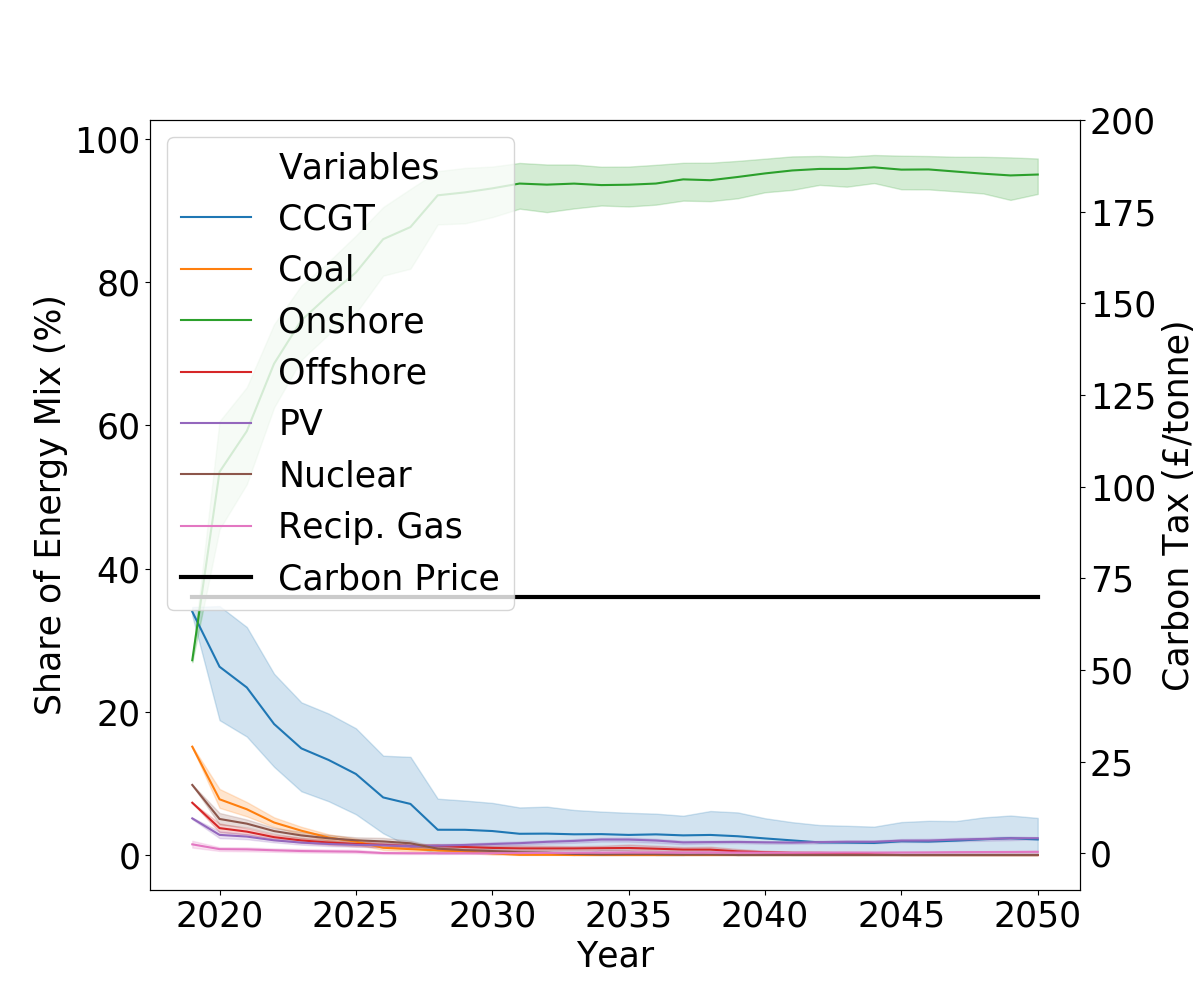
\includegraphics[width=0.5\textwidth]{figures/scenarios/demand099-carbon70-datetime.png}
		\caption{Demand decreasing by 1\% per year with a carbon tax of \textsterling20}
		\label{fig:demand99carbon70}
	\end{center}
\end{figure}



\begin{figure*}[h]
	\centering
	\begin{subfigure}[b]{0.475\textwidth}
		\centering
		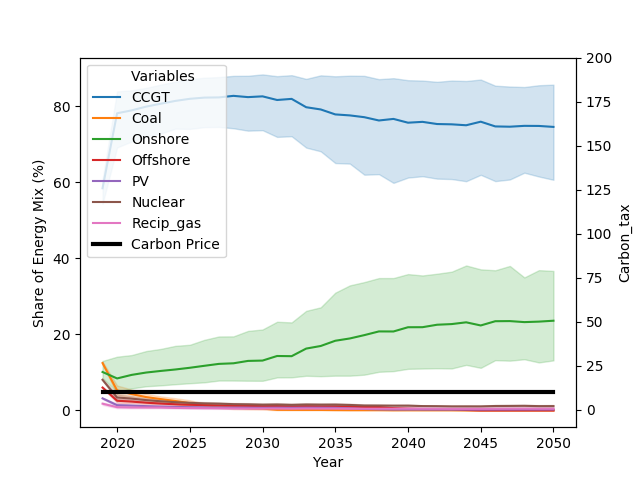
\includegraphics[width=\textwidth]{figures/scenarios/demand099-carbon10-datetime.png}
		\caption[Network2]%
		{{\small \textsterling10 carbon tax.}}    
		\label{fig:demand99carbon10}
	\end{subfigure}
	\hfill
	\begin{subfigure}[b]{0.475\textwidth}  
		\centering 
		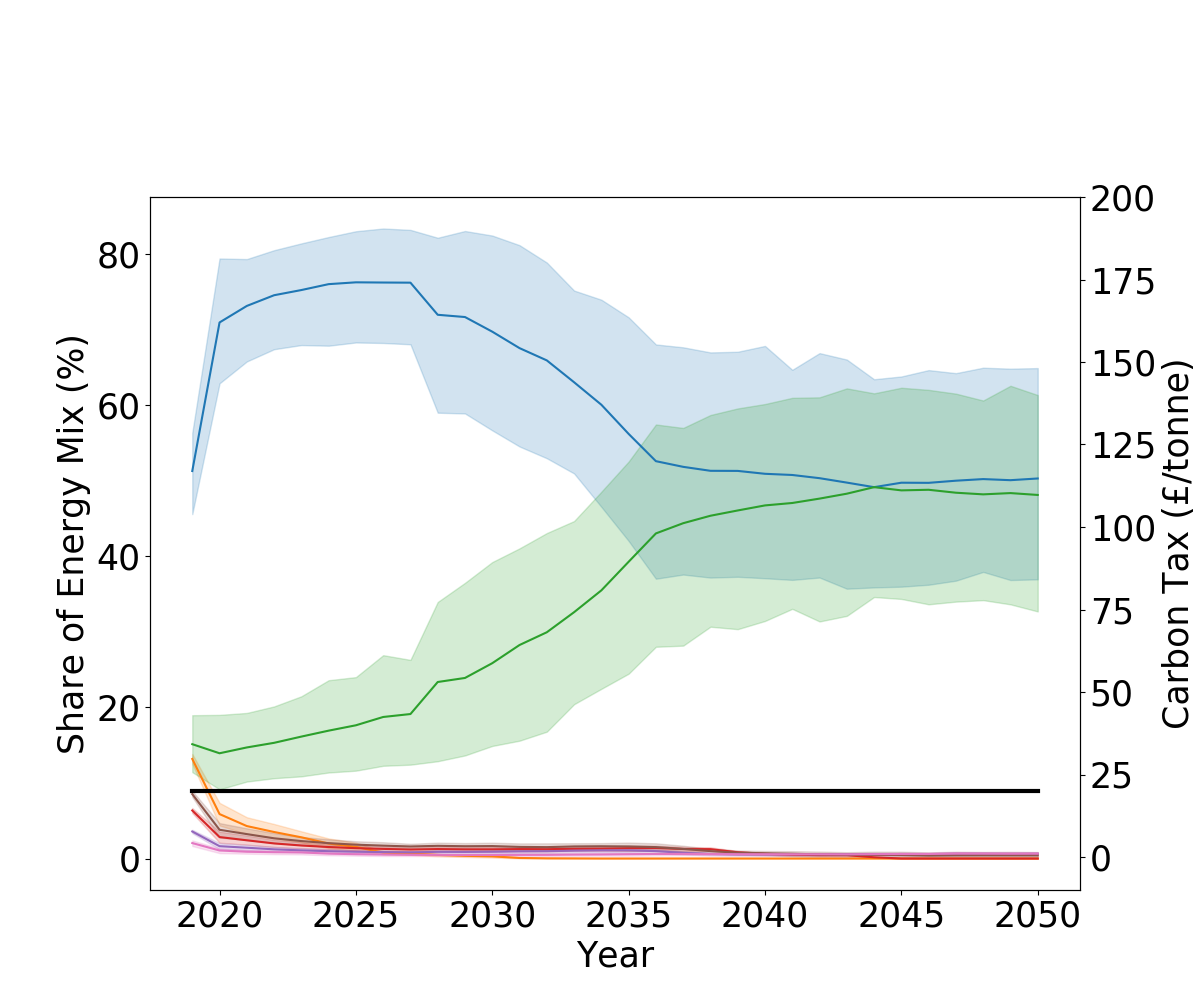
\includegraphics[width=\textwidth]{figures/scenarios/demand099-carbon20-datetime.png}
		\caption[]%
		{{\textsterling20 carbon tax.}}    
		\label{fig:demand99carbon20}
	\end{subfigure}
	\vskip\baselineskip

	\begin{subfigure}[b]{0.475\textwidth}   
		\centering 
		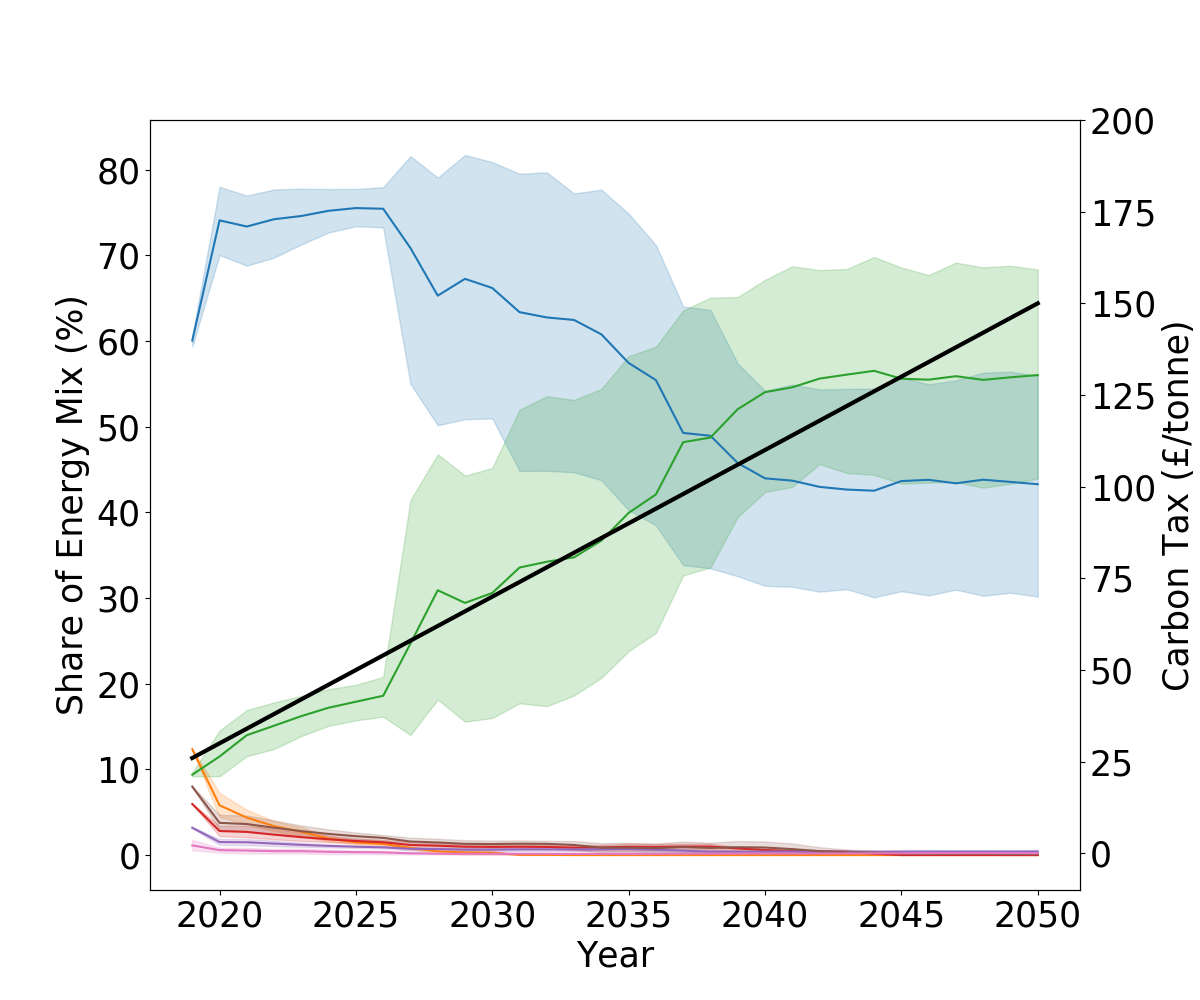
\includegraphics[width=\textwidth]{figures/scenarios/demand099-carbon18-datetime.png}
		\caption[]%
		{{\textsterling26 to \textsterling150 linearly increasing carbon tax.}}    
		\label{fig:demand99carbon18}
	\end{subfigure}
	\quad
	\begin{subfigure}[b]{0.475\textwidth}   
		\centering 
		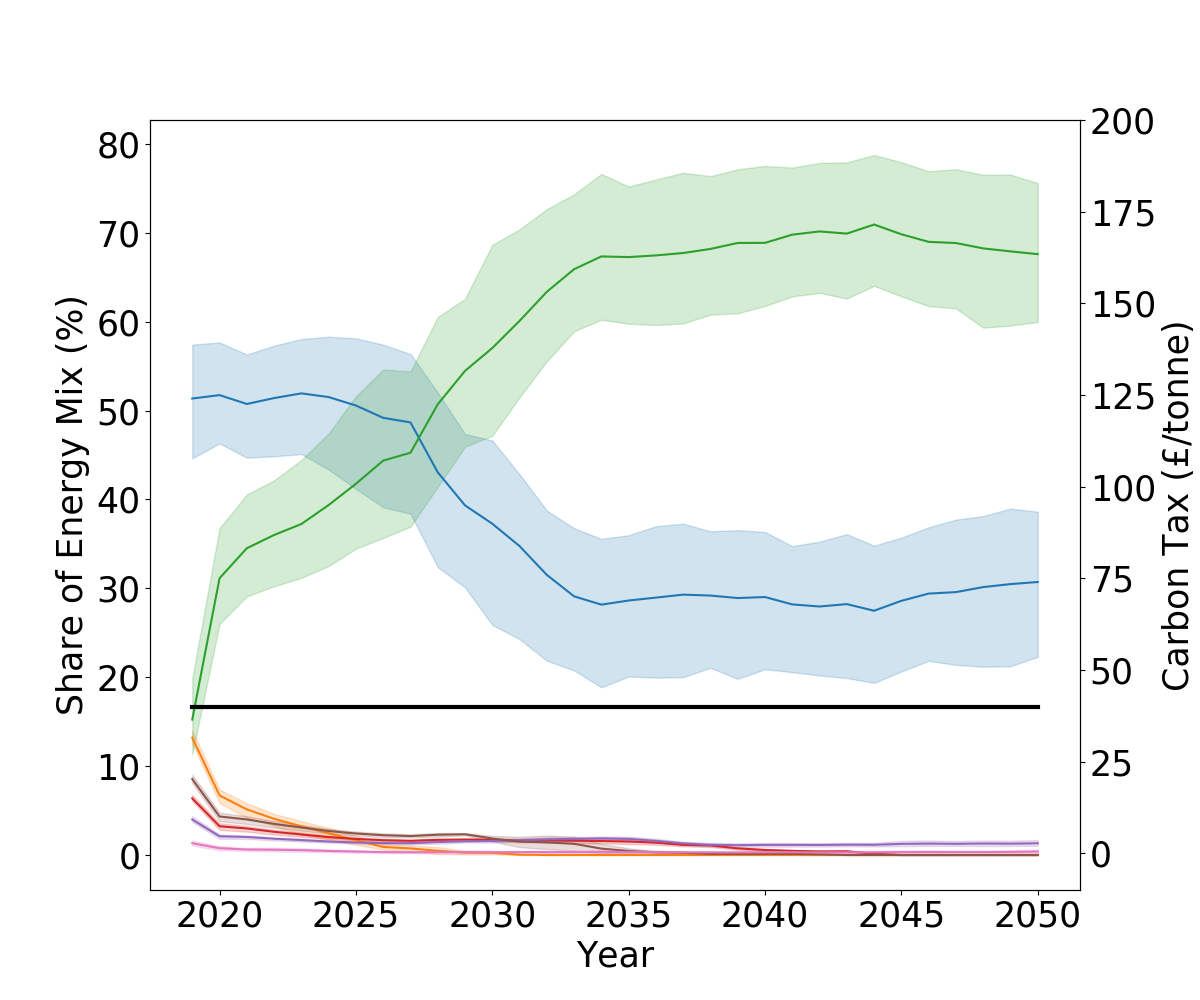
\includegraphics[width=\textwidth]{figures/scenarios/demand099-carbon40-datetime.png}
		\caption[]%
		{{\textsterling40 carbon tax.}}    
		\label{fig:demand99carbon40}
	\end{subfigure}
	\caption[ Scenarios up to the year 2050 with varying carbon taxes and decreasing demand ]
	{\small Scenarios up to the year 2050, with varying carbon taxes and electricity demand decreasing 1\% a year.} 
	\label{fig:mean and std of nets}
\end{figure*}
%\FloatBarrier








%\begin{figure}[h]
%	\begin{center}
%		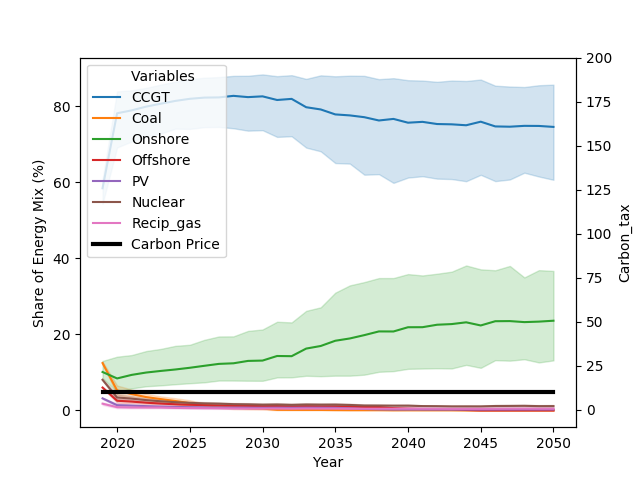
\includegraphics[width=0.5\textwidth]{figures/scenarios/demand099-carbon10-datetime.png}
%		\caption{Demand decreasing by 1\% per year and a carbon tax of \textsterling10}
%		\label{fig:demand99carbon10}
%	\end{center}
%\end{figure}
%
%\begin{figure}[h]
%	\begin{center}
%		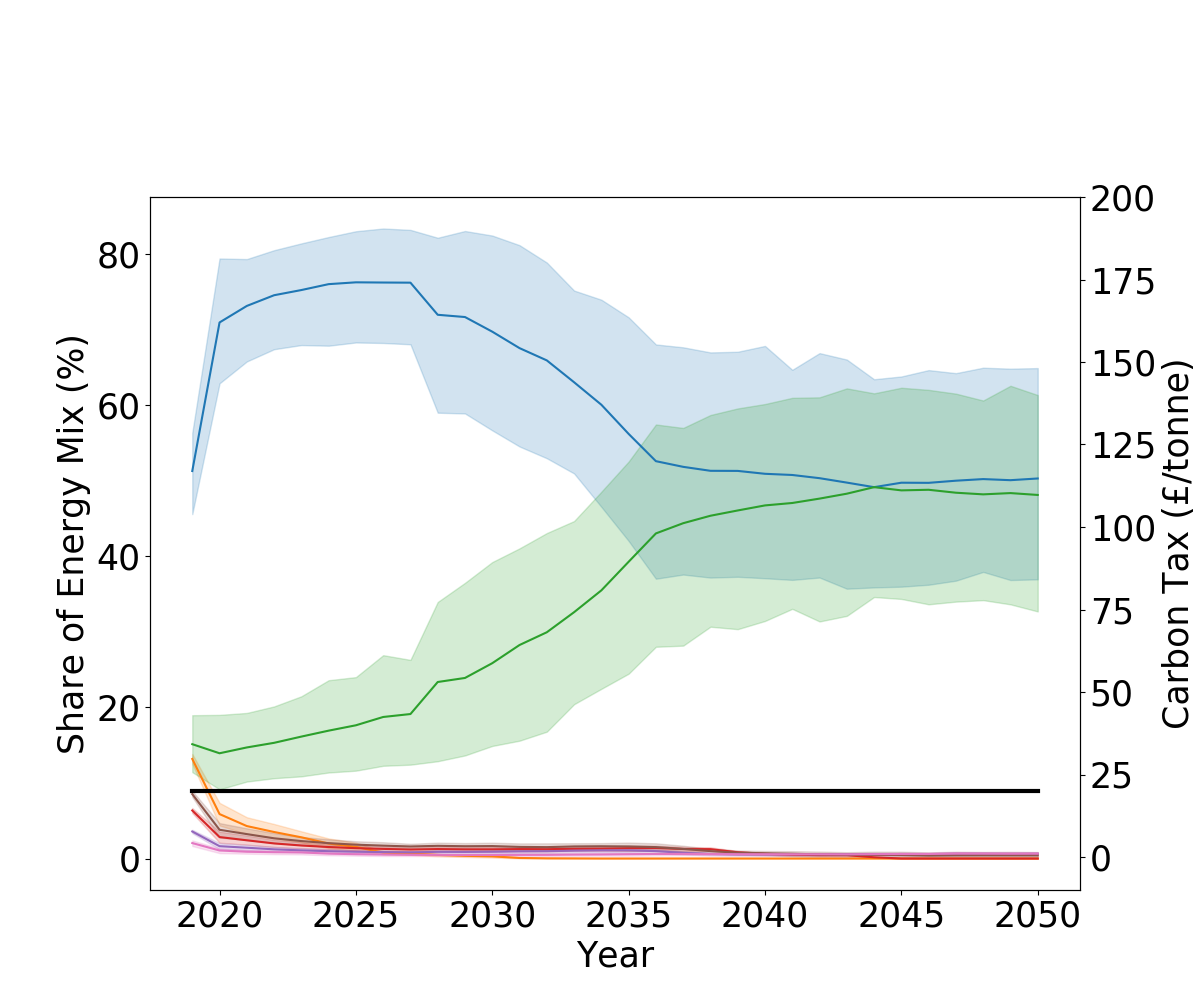
\includegraphics[width=0.5\textwidth]{figures/scenarios/demand099-carbon20-datetime.png}
%		\caption{Demand decreasing by 1\% per year and a carbon tax of \textsterling20}
%		\label{fig:demand99carbon10}
%	\end{center}
%\end{figure}
%
%
%
%\begin{figure}[h]
%	\begin{center}
%		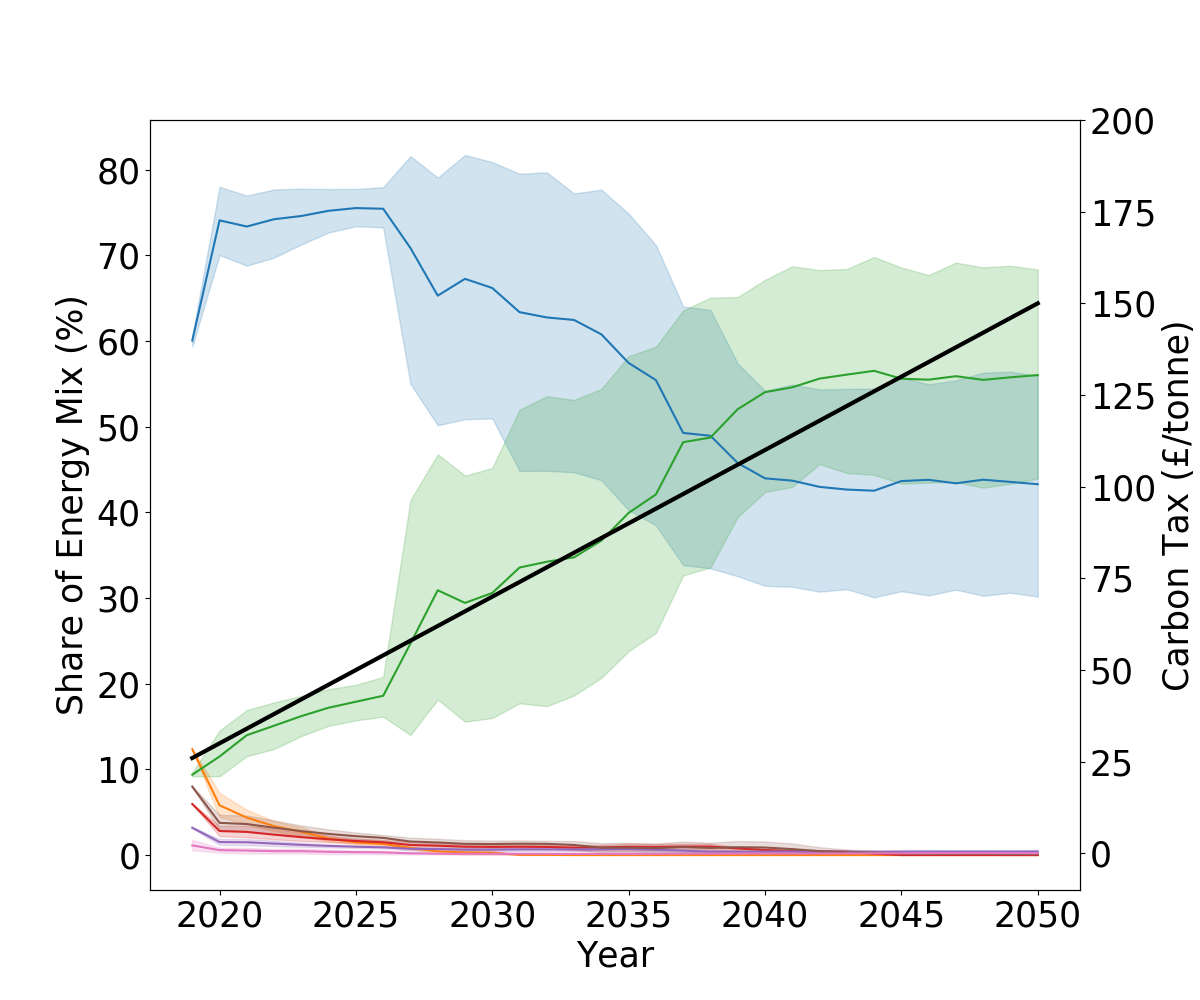
\includegraphics[width=0.5\textwidth]{figures/scenarios/demand099-carbon18-datetime.png}
%		\caption{Demand decreasing by 1\% per year and a carbon tax of \textsterling20}
%		\label{fig:demand99carbon10}
%	\end{center}
%\end{figure}
%
%
%
%\begin{figure}[h]
%	\begin{center}
%		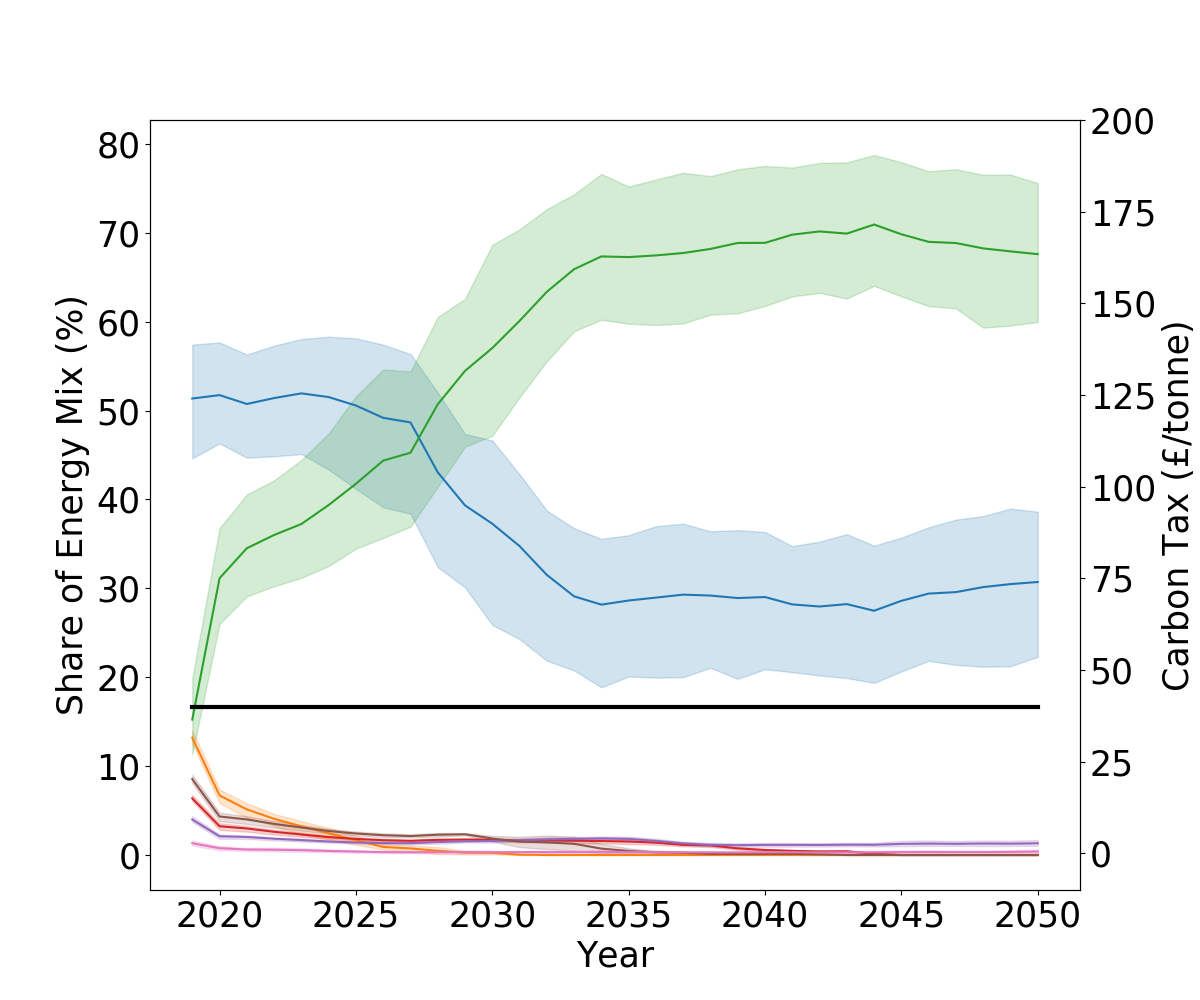
\includegraphics[width=0.5\textwidth]{figures/scenarios/demand099-carbon40-datetime.png}
%		\caption{Demand decreasing by 1\% per year and a carbon tax of \textsterling20}
%		\label{fig:demand99carbon10}
%	\end{center}
%\end{figure}











%\begin{itemize}
%	\item Effect of different carbon tax on investments made.
%	\item Effects of different demand scenarios. (High peaks, high growth, high reduction in demand)
%	\item Effects of high fuel prices.
%	\item Different costs of capital (eg. Borrowing for Nuclear of interest rate to equal 2\% at government bonds rate, as opposed to 10\% for private companies.)
%	\item Different learning rates for renewable costs.
%	\item The effect of long term carbon tax policy (eg. Carbon price known for next 25 years) vs short term changes in carbon tax.
%\end{itemize}




\section{Conclusions}\label{Conclusion}

\begin{itemize}
	\item Requirement for agent based models based on imperfect information, liberalised energy markets
	\item Requirement for low barriers to entry open source model.
	\item Discuss results
	\item Future work:
	\begin{itemize}
		\item Embedding multi-agent intelligence such as Genetic Algorithms,  Q-learning and dynamic reinforcement learning
		\item Raise spatial and temporal resolution.
	\end{itemize}
\end{itemize}






%
% The acknowledgments section is defined using the "acks" environment (and NOT an unnumbered section). This ensures
% the proper identification of the section in the article metadata, and the consistent spelling of the heading.
\begin{acks}
To Robert, for the bagels and explaining CMYK and color spaces.
\end{acks}

%
% The next two lines define the bibliography style to be used, and the bibliography file.
\bibliographystyle{ACM-Reference-Format}
\bibliography{library,custombibtex}

% 
% If your work has an appendix, this is the place to put it.
\appendix

\section{Research Methods}

\subsection{Parameters}

\begin{table*}[]
	\begin{tabular}{|l|l|l|l|l|l|l|l|l|l|l|l|l|l|}
		\hline
		Type          & Plant\_Size & year             & $\eta$ & $OP$ & $P_D$ & $C_D$ & $P_C$    & $C_C$     & $I_C$    & $F_C$   & $V_C$ & $In_C$  & $Con_C$  \\ \hline
		CCGT          & 168.0       & 2018, 2020, 2025 & 0.34   & 25.0 & 3     & 3     & 60000.0  & 700000.0  & 13600.0  & 28200.0 & 5.0   & 2900.0  & 3300.0   \\ \hline
		CCGT          & 1200.0      & 2018, 2020, 2025 & 0.54   & 25.0 & 3     & 3     & 10000.0  & 500000.0  & 15100.0  & 12200.0 & 3.0   & 2100.0  & 3300.0   \\ \hline
		CCGT          & 1471.0      & 2018, 2020, 2025 & 0.53   & 25.0 & 3     & 3     & 10000.0  & 500000.0  & 15100.0  & 11400.0 & 3.0   & 1900.0  & 3300.0   \\ \hline
		Coal          & 552.0       & 2025             & 0.32   & 25.0 & 6     & 6     & 40000.0  & 3400000.0 & 10000.0  & 68200.0 & 6.0   & 13000.0 & 3800.0   \\ \hline
		Coal          & 624.0       & 2025             & 0.32   & 25.0 & 5     & 5     & 70000.0  & 4200000.0 & 10000.0  & 79600.0 & 3.0   & 19300.0 & 3800.0   \\ \hline
		Coal          & 652.0       & 2025             & 0.3    & 25.0 & 5     & 5     & 60000.0  & 3900000.0 & 10000.0  & 65300.0 & 5.0   & 22700.0 & 3800.0   \\ \hline
		Coal          & 734.0       & 2025             & 0.38   & 25.0 & 5     & 5     & 60000.0  & 2600000.0 & 10000.0  & 56400.0 & 3.0   & 9600.0  & 3800.0   \\ \hline
		Coal          & 760.0       & 2025             & 0.35   & 25.0 & 5     & 5     & 40000.0  & 2800000.0 & 10000.0  & 52100.0 & 5.0   & 14000.0 & 3800.0   \\ \hline
		Hydro         & 0.033       & 2018, 2020, 2025 & 1.0    & 35.0 & 0     & 0     & 0.0      & 6300000.0 & 0.0      & 83300.0 & 0.0   & 0.0     & 0.0      \\ \hline
		Hydro         & 1.046       & 2018, 2020, 2025 & 1.0    & 35.0 & 0     & 0     & 0.0      & 3300000.0 & 400.0    & 18200.0 & 0.0   & 0.0     & 0.0      \\ \hline
		Hydro         & 11.0        & 2018, 2020, 2025 & 1.0    & 41.0 & 2     & 2     & 60000.0  & 3000000.0 & 0.0      & 45100.0 & 6.0   & 0.0     & 0.0      \\ \hline
		Nuclear       & 3300.0      & 2025             & 1.0    & 60.0 & 5     & 8     & 240000.0 & 4100000.0 & 11500.0  & 72900.0 & 5.0   & 10000.0 & 500.0    \\ \hline
		OCGT          & 96.0        & 2018, 2020, 2025 & 0.35   & 25.0 & 2     & 2     & 80000.0  & 600000.0  & 12600.0  & 9900.0  & 4.0   & 2500.0  & 2400.0   \\ \hline
		OCGT          & 299.0       & 2018, 2020, 2025 & 0.35   & 25.0 & 2     & 2     & 30000.0  & 400000.0  & 13600.0  & 9600.0  & 3.0   & 1600.0  & 2500.0   \\ \hline
		OCGT          & 311.0       & 2018, 2020, 2025 & 0.35   & 25.0 & 2     & 2     & 30000.0  & 400000.0  & 13600.0  & 9500.0  & 3.0   & 1600.0  & 2500.0   \\ \hline
		OCGT          & 400.0       & 2018, 2020, 2025 & 0.34   & 25.0 & 2     & 2     & 30000.0  & 300000.0  & 15100.0  & 7800.0  & 3.0   & 1300.0  & 2500.0   \\ \hline
		OCGT          & 625.0       & 2018, 2020, 2025 & 0.35   & 25.0 & 2     & 2     & 20000.0  & 300000.0  & 15100.0  & 4600.0  & 3.0   & 1200.0  & 2400.0   \\ \hline
		OCGT\_CCS     & 290.0       & 2025             & 0.24   & 25.0 & 5     & 5     & 80000.0  & 2300000.0 & 15100.0  & 31800.0 & 3.0   & 8500.0  & 2500.0   \\ \hline
		Offshore      & 321.0       & 2018             & 0.0    & 23.0 & 5     & 3     & 60000.0  & 2200000.0 & 69300.0  & 30900.0 & 3.0   & 1400.0  & 33500.0  \\ \hline
		Offshore      & 321.0       & 2020             & 0.0    & 23.0 & 5     & 3     & 60000.0  & 2100000.0 & 69300.0  & 30000.0 & 3.0   & 1400.0  & 32600.0  \\ \hline
		Offshore      & 321.0       & 2025             & 0.0    & 23.0 & 5     & 3     & 60000.0  & 1900000.0 & 69300.0  & 28600.0 & 3.0   & 1300.0  & 31100.0  \\ \hline
		Offshore      & 844.0       & 2018             & 0.0    & 22.0 & 5     & 3     & 120000.0 & 2400000.0 & 323000.0 & 48600.0 & 4.0   & 3300.0  & 50300.0  \\ \hline
		Offshore      & 844.0       & 2020             & 0.0    & 22.0 & 5     & 3     & 120000.0 & 2300000.0 & 323000.0 & 47300.0 & 3.0   & 3300.0  & 48900.0  \\ \hline
		Offshore      & 844.0       & 2025             & 0.0    & 22.0 & 5     & 3     & 120000.0 & 2100000.0 & 323000.0 & 45400.0 & 3.0   & 3100.0  & 47000.0  \\ \hline
		Onshore       & 0.01        & 2018             & 1.0    & 20.0 & 0     & 0     & 0.0      & 3700000.0 & 0.0      & 29700.0 & 0.0   & 0.0     & 0.0      \\ \hline
		Onshore       & 0.01        & 2020             & 1.0    & 20.0 & 0     & 0     & 0.0      & 3600000.0 & 0.0      & 29600.0 & 0.0   & 0.0     & 0.0      \\ \hline
		Onshore       & 0.01        & 2025             & 1.0    & 20.0 & 0     & 0     & 0.0      & 3500000.0 & 0.0      & 29600.0 & 0.0   & 0.0     & 0.0      \\ \hline
		Onshore       & 0.482       & 2018             & 1.0    & 20.0 & 0     & 0     & 0.0      & 2200000.0 & 200.0    & 56900.0 & 0.0   & 0.0     & 0.0      \\ \hline
		Onshore       & 0.482       & 2020             & 1.0    & 20.0 & 0     & 0     & 0.0      & 2100000.0 & 200.0    & 56900.0 & 0.0   & 0.0     & 0.0      \\ \hline
		Onshore       & 0.482       & 2025             & 1.0    & 20.0 & 0     & 0     & 0.0      & 2000000.0 & 200.0    & 56700.0 & 0.0   & 0.0     & 0.0      \\ \hline
		Onshore       & 20.0        & 2018             & 0.0    & 24.0 & 4     & 2     & 110000.0 & 1200000.0 & 3300.0   & 23200.0 & 5.0   & 1400.0  & 3100.0   \\ \hline
		Onshore       & 20.0        & 2020             & 0.0    & 24.0 & 4     & 2     & 110000.0 & 1200000.0 & 3300.0   & 23000.0 & 5.0   & 1400.0  & 3100.0   \\ \hline
		Onshore       & 20.0        & 2025             & 0.0    & 24.0 & 4     & 2     & 110000.0 & 1200000.0 & 3300.0   & 22400.0 & 5.0   & 1400.0  & 3000.0   \\ \hline
		PV            & 0.003       & 2018             & 1.0    & 30.0 & 0     & 0     & 0.0      & 1500000.0 & 0.0      & 23500.0 & 0.0   & 0.0     & 0.0      \\ \hline
		PV            & 0.003       & 2020             & 1.0    & 30.0 & 0     & 0     & 0.0      & 1500000.0 & 0.0      & 23400.0 & 0.0   & 0.0     & 0.0      \\ \hline
		PV            & 0.003       & 2025             & 1.0    & 30.0 & 0     & 0     & 0.0      & 1400000.0 & 0.0      & 23200.0 & 0.0   & 0.0     & 0.0      \\ \hline
		PV            & 0.455       & 2018             & 1.0    & 30.0 & 0     & 0     & 0.0      & 1000000.0 & 200.0    & 9400.0  & 0.0   & 0.0     & 0.0      \\ \hline
		PV            & 0.455       & 2025             & 1.0    & 30.0 & 0     & 0     & 0.0      & 900000.0  & 200.0    & 9200.0  & 0.0   & 0.0     & 0.0      \\ \hline
		PV            & 1.0         & 2018             & 0.0    & 25.0 & 1     & 0     & 20000.0  & 700000.0  & 0.0      & 6600.0  & 3.0   & 2600.0  & 1300.0   \\ \hline
		PV            & 1.0         & 2020             & 0.0    & 25.0 & 1     & 0     & 20000.0  & 700000.0  & 0.0      & 6300.0  & 3.0   & 2600.0  & 1300.0   \\ \hline
		PV            & 1.0         & 2025             & 0.0    & 25.0 & 1     & 0     & 20000.0  & 600000.0  & 0.0      & 5900.0  & 3.0   & 2400.0  & 1200.0   \\ \hline
		PV            & 4.0         & 2018             & 0.0    & 25.0 & 1     & 0     & 60000.0  & 700000.0  & 200.0    & 8300.0  & 0.0   & 1200.0  & 1300.0   \\ \hline
		PV            & 4.0         & 2020             & 0.0    & 25.0 & 1     & 0     & 60000.0  & 700000.0  & 200.0    & 8000.0  & 0.0   & 1100.0  & 1300.0   \\ \hline
		PV            & 4.0         & 2025             & 0.0    & 25.0 & 1     & 0     & 60000.0  & 600000.0  & 200.0    & 7500.0  & 0.0   & 1100.0  & 1200.0   \\ \hline
		PV            & 16.0        & 2018             & 0.0    & 25.0 & 1     & 0     & 70000.0  & 700000.0  & 400.0    & 5600.0  & 0.0   & 2000.0  & 1300.0   \\ \hline
		PV            & 16.0        & 2020             & 0.0    & 25.0 & 1     & 0     & 70000.0  & 600000.0  & 400.0    & 5400.0  & 0.0   & 1900.0  & 1300.0   \\ \hline
		PV            & 16.0        & 2025             & 0.0    & 25.0 & 1     & 0     & 70000.0  & 600000.0  & 400.0    & 5100.0  & 0.0   & 1800.0  & 1200.0   \\ \hline
		Recip\_diesel & 20.0        & 2018, 2020, 2025 & 0.34   & 15.0 & 2     & 1     & 10000.0  & 300000.0  & 2200.0   & 10000.0 & 2.0   & 1000.0  & -31900.0 \\ \hline
		Recip\_gas    & 20.0        & 2018, 2020, 2025 & 0.32   & 15.0 & 2     & 1     & 10000.0  & 300000.0  & 3400.0   & 10000.0 & 2.0   & 1000.0  & -31900.0 \\ \hline
	\end{tabular}
\end{table*}



\end{document}
